\chapter{Graph Attention Networks Embedded Knowledge Tracing Model With Transformer}

% **************************** Define Graphics Path **************************
\ifpdf
    \graphicspath{{Chapter3/Figs/Raster/}{Chapter3/Figs/PDF/}{Chapter3/Figs/}}
\else
    \graphicspath{{Chapter3/Figs/Raster/}{Chapter3/Figs/Vector/}{Chapter3/Figs/PDF/}{Chapter3/Figs/}}
\fi

\section{Research Motivation}
%本章节为该推荐系统的一个核心部分,即通过知识追踪的方式获取学生的知识掌握状态。该模型用于评估学生的知识掌握状态,在后续的推荐模型中作为推荐的基础依据。知识追踪是一种常见的用于学生的认知诊断的模型,它根据学生的以往的答题记录来建模学生的知识掌握情况,从而获取学生的知识状态。知识追踪的模型非常丰富,早期的知识追踪模型贝叶斯知识追踪(BKT),它们的基础假设是学生答题基于一系列知识点,这些知识点之间被认为是相互不相关的,因此它们之间是独立表示,这种做法无法捕捉不同概念之间的关系也无法表征复杂的概念转换。在2015年,Piech等人提出了深度知识追踪模型(DKT),首次将长短期记忆网络(LSTM)应用于知识追踪任务,它无需进行知识点标注,而是包含一个知识的隐含状态,当时取得了超过BKT的基线性能,它标志着基于神经网络模型的知识追踪研究的序幕。但DKT无法输出知识的隐藏状态,可解释性不足。而且DKT用将所有记忆存储于一个隐藏向量中,对于长序列的预测性能不够理想。针对这个问题,记忆增强网络(MANN)被提出来,它允许网络保留多个隐藏状态向量,并分别读写这些向量。在2017年,张等人提出了Dynamic Key-Value Memory Networks(DKVMN),它参考了MANN的设计,针对知识追踪任务进行了优化,优化了MANN对于知识追踪任务的输入输出不同域的问题。DKVMN采用了键值对作为存储器结构,能避免过拟合、参数少,以及通过潜在概念自动发现相似练习,取得了相对BKT和DKT更好的预测性能。同时该模型也具有较好的可解释性,它将问题相关潜在概念存储于键矩阵中,对概念掌握程度存储于值矩阵中,通过对输入练习与键矩阵的相关性对值矩阵进行更新。

%尽管该模型取得了较好的性能,但该模型将知识点建模为相互独立的点,而未考虑知识点之间的关联性。在高中数学知识网络中,知识点与知识点间有网状的关联关系,而习题是基于这些知识点建立的。因此习题与习题之间也存在隐含的间接关联关系,因此设计一种将考虑知识点间关联的模型来表征该模型是一种合理的解决方案。除了考虑习题知识点的掌握程度,对于学生的答题行为也可以作为额外的特征加入该模型,这样可以为模型增加更多的考虑因素,从而增强模型的预测性能。本文提出了一种用图神经网络结合记忆增强网络的知识追踪模型。该模型相对于原始的DKVMN模型,用图神经网络改造了知识点表征矩阵,并将学生的额外答题行为特征作为模型输入。

This section is a core part of this recommendation system to obtain the student's knowledge mastery status using knowledge tracing. The model is used to assess the student's knowledge acquisition status, which is used as the basis for recommendations in the subsequent recommendation model. Knowledge tracing is a common model used for cognitive diagnosis of students, which models students' knowledge acquisition based on their previous answer records to obtain their knowledge status~\cite{gonzalez2014general}. There is a wealth of models for knowledge tracing, early models of knowledge tracing Bayesian Knowledge Tracing (BKT)~\cite{yudelson2013individualized}, which issued the assumption that students' solutions to exercises are based on a set of knowledge points that are considered to be unrelated to each other and are therefore represented independently of each other. This approach fails to capture the relationships between different concepts nor to characterize complex conceptual transformations. In 2015, Piech et al. proposed the deep knowledge tracing model (DKT), which first applied RNN to the knowledge tracing task, which contains an implicit state of knowledge, and achieved a baseline performance over BKT at that time, and it marked the prologue of knowledge tracing research based on neural network models. However, DKT cannot output the hidden state of knowledge and is not sufficiently interpretable.

Moreover, DKT uses to store all memories in a hidden vector, and the prediction performance for long sequences is not satisfactory enough. Memory Augmented Neural Network (MANN)~\cite{santoro2016meta} was proposed to address this problem, which allows the network to keep multiple hidden state vectors and read and write these vectors separately. In 2017, Dynamic Key-Value Memory Networks (DKVMN)~\cite{zhang2017dynamic} referring to the design of MANN for knowledge tracing tasks and optimizes MANN for knowledge tracing tasks with different input and output domains. DKVMN uses key-value pairs as the memory structure, which can avoid over better prediction performance relative to BKT, and DKT is achieved by using key-value pairs as the memory structure, which can avoid overfitting. The model also has better interpretability. It stores the problem-related potential concepts in the key matrix and the mastery proficiency to the concepts in the value matrix and updates the value matrix by correlating the input exercises with the key matrix.

Although the model achieved better performance, the model modeled knowledge points as mutually independent points without considering the correlations. There are web-like correlations between knowledge points in the high school mathematics knowledge network, and the exercises are built based on these knowledge points. Therefore, there are also implicit and indirect correlations between the exercises and the exercises, so it is reasonable to design a model that will consider the correlations between knowledge points to characterize the model. In addition to considering the degree of mastery of the exercises' knowledge points, the students' answering behaviors can also be added to the model as additional features, adding more consideration to the model and enhancing the model's predictive performance. This thesis proposes a knowledge tracing model using graph neural networks combined with memory enhancement networks. The model transforms the knowledge point representation matrix with graph neural networks relative to the original DKVMN model and uses additional characteristics of students' answering behaviors as model inputs.

\section{Research Contribution}
%DKVMN模型有如下的问题,第一,该模型未考虑学生的特性,每个学生对于潜在知识点的掌握程度会导致不同的结果,即,当两个知识点掌握程度相同的学生可能对于一个习题的作答结果会产生不同的预测度。第二,该模型未考虑知识点的内在联系,该模型将知识点作为存储结构中的一个slot,各个slot之间相互独立。这隔绝了知识点变化引起的相关知识点的变化。在高中数学学科中,有许多相互相关的知识点,因此,需要结合领域特征,加入知识点关联学习网络。本文基于上述两点,对DKVMN模型进行改进。
In this section, an improved knowledge tracing model is proposed based on the DKVMN structure. The DKVMN model is improved based on the above two points. The DKVMN model has the following problems. First, the model does not take into account the characteristics of students, and each student's mastery of potential knowledge points will lead to different results, i.e., when two students with the same level of mastery of knowledge points may have different prediction degrees for the answer results of an exercise. Second, the model does not consider the intrinsic connection of the knowledge points, which are treated as a slot in the storage structure, and each slot is independent of others. This prevents the changes in related knowledge points caused by changes in knowledge points. In high school mathematics subjects, there are many interrelated knowledge points. Therefore, it is necessary to incorporate the domain characteristics and join the knowledge point associated learning network.

\section{Related Theory}
\subsection{Knowledge Tracing}
%知识追踪为智能化和自适应教育提供了条件,它具有个性化和自动化的特点。知识追踪任务从学生的历史学习记录来追踪学生的知识状态变化,预测未来的学习表现,从而针对性地给予学习辅导。其本质基于学生的过去的学习表现来获取当前的学习状态,从而预测将来的学习表现。其实际做法是,对学生过去的答题记录进行数据分析和过程建模,从而建模当前的学生学习状态数据,让模型跟做学生的每个阶段的学习状态,并基于学习状态数据来预测习题答对的概率。在学科学习中,学科知识由一系列知识点组成,学生的学习状态实际上基于对于各个知识点的掌握情况。而知识追踪一般的形式为给定一个学生的答题序列,该序列由一系列习题构成,习题又与特定的知识点相关联,在知识追踪中的一个基本假设是,学生的答题表现基于对知识点的掌握。而学生的答题表现即可用于反推学生对于各个知识点的掌握情况,即学习状态的掌握情况。

%知识追踪任务的数学表示为一个学生在一个习题序列上的交互式答题记录\(X_t=(x_1,x_2,\ldots,x_t)\),根据该记录通过建模来获取学生的学习状态,并预测学生在下一次练习中的表现$x_{t+1}$。其中$x_t$通常表示为一个有序对$(q_t,a_t)$,有序对表示学生在时间$t$回答了问题$q_t$,$a_t$表示问题的得分情况,也有许多知识追踪任务用答对或答错来表示,此时$a_t$为0或者1,在此情况下,实际上预测的是对于下一个问题回答正确的概率$P(a_{t+1}=1|a_t)$。如图ref{kt1}。

Knowledge tracing provides the conditions for intelligent and adaptive education, which is personalized and automated. Knowledge tracing tracks students' knowledge status from their historical learning records, predicts future learning performance and provides targeted learning coaching. The essence is to obtain the current learning status based on the student's past learning performance to predict the future learning performance. The actual practice is to analyze the data and process modeling of students' past answer records to model the current student learning status data and let the model follow the learning status of students at each stage, and predict the probability of correct answers to the exercises based on the learning status data. In subject learning, subject knowledge consists of a series of knowledge points, and students' learning status is based on their mastery proficiency to each elementary knowledge concept. The general form of knowledge tracing is that given a sequence of student answers, which consists of a series of exercises associated with a specific knowledge point, a fundamental assumption in knowledge tracing is that student performance is based on mastery proficiency to the knowledge concept. The student's performance can be applied to infer the student's mastery proficiency for each knowledge concept, i.e., the mastery proficiency to the learning state.

The mathematical representation of the knowledge tracing task is an interactive answer record \(X_t=(x_1,x_2,\ldots,x_{t-1})\) of a student on an exercise sequence, based on which the student's learning status is obtained by modeling and predicting the student's performance in the next exercise \(x_{t}\). Where \(x_t\) is usually represented as an ordered pair \((q_t,a_t)\), the ordered pair indicates that the student answered the exercise \(q_t\) at time \(t\), and \(a_t\) indicates the score of the exercise, also many knowledge tracing tasks are represented by correct or incorrect answers, when \(a_t\) is 0 or 1. In this case, what is actually predicted is the probability of answering correctly for the next exercise \(P(a_{t}=1|a_{t-1},\ldots,a_1)\). As shown in the figure \figname{\ref{fig:ch3-model-ktdes}}.

\begin{figure}[htbp!]
    \centering
    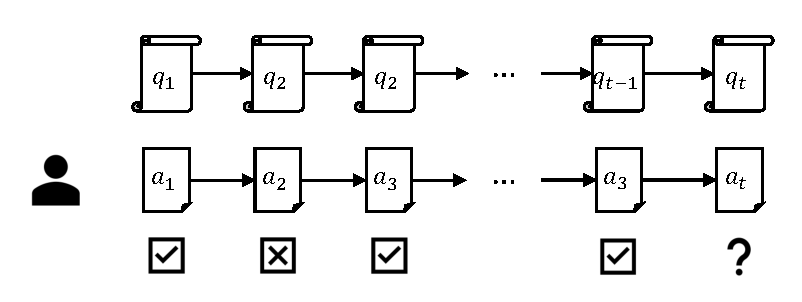
\includegraphics[width=0.9\textwidth]{ch3-kt-model.pdf}
    \caption{The knowledge tracing pattern}\label{fig:ch3-model-ktdes}
\end{figure}

\subsection{Dynamic Key-Value Memory Networks}
%在传统的机器学习模型中,逻辑流控制和外部记忆机制往往缺失。因此,许多当前的机器学习模型无法建立复杂的逻辑流控制和外部记忆模块。传统的模型往往无法高效地利用可训练参数来获得较强记忆能力的模型。目前像LSTM和GRU这些结构,具备一定的记忆能力,但该能力受可训练参数数目影响,记忆增强网络通过更强的表征能力来摆脱可训练参数数目与模型的记忆能力之间的联系。它能够模拟人脑的工作记忆机制,例如阅读理解、推理、运算过程等,也可以捕捉复杂的结构信息和建立长距离信息依赖。MANN将中间信息保留在内存中,形成一个信息缓存结构,并利用该信息进行后续的推理学习。在一个MANN网络中往往分为控制器、存储模块和读写器等三个部分。控制器读取前一阶段的状态和当前的输入来获取下一阶段的输出和控制器输出。存储模块是一个数据结构模型,例如栈、队列或数组,每一个时刻都通过一个输出函数处理读取内容和控制器输出来计算序列输出。

%在知识追踪任务中,由于习题所包含的知识点表征与知识点掌握状态表征所处的空间不同,因此无法将掌握程度和知识点表征用一个存储结构来保存,因此需要对MANN模型进行改造来适配知识追踪任务。DKVMN通过将知识点表征保存在一个矩阵\(M^{(k)}\)中作为Keys,将对应知识点掌握表征保存在另一个矩阵\(M^{(v)}\)中,作为Values。在输入一个习题表示\(q_t\)时,模型将\(q_t\)的嵌入表示向量\(k_t\)与知识点表征模块\(M^{(k)}\)进行相关度计算,得到习题的知识点相关度表示向量\(w_t\)。每个习题都可以表示为一个与知识点的相关度向量,代表了与知识点的相互关系。在DKVMN模型中,有读取过程和写入过程。

%在读取过程中,模型将权重向量\(w_t\)与知识点掌握矩阵\(M^{(v)}\)进行加权和计算,获得用户对于知识点的掌握表征向量\(r_t\)。并将\(r_t\)与当前的习题嵌入向量\(k_t\)进行拼接,经过全联接激活层输\(Tanh(\cdot)\)出\(f_t\),它表示用户对于习题的掌握程度。\(f_t\)会经过一个最终的\(Sigmoid(\cdot)\)激活函数来输出一个习题回答正确的预测概率\(p_t\)。在写入过程中,当前的实际回答表现会对学生的知识掌握状态产生影响,这是一个重新评估的过程。当前的交互记录\(x_t=(q_t,a_t)\)会作为模型的输入。它的嵌入表示\(v_t\)会用于计算知识减少向量\(e_t\)与知识增加向量\(a_t\),减少向量与增加向量会经过与\(w_t\)的加权和作用于\(M^{(v)}\)从而实现对于学生知识状态的更改。训练国歌通过最小化\(p_t\)与习题作答正确性真实标签\(a_t\)的交叉熵损失来进行。整个模型是可微的,因此可以有效利用随机梯度下降来训练。

In traditional machine learning models, logic flow control and external memory mechanisms are often missing. As a result, many current machine learning models cannot build complex logic flow control and external memory modules. Traditional models are often unable to efficiently use trainable parameters to obtain models with strong memory capabilities. Current structures like LSTM and GRU have some memory capability, but that capability is affected by trainable parameters. MANN gets rid of the connection between the number of trainable parameters and the model's memory capability by more robust representational capability. It can simulate the human brain's working memory mechanisms, such as reading comprehension, reasoning, and arithmetic processes, and capture complex structural information and establish long-range information dependencies. MANN keeps intermediate information in memory, forming an information cache structure, and uses that information for subsequent reasoning learning. A MANN network is commonly divided into three parts such as controller, storage module, and reader. The controller reads the previous stage's state and the current input to obtain the next stage's output and the controller output. The storage module is a data structure model, such as a stack, queue, or array, and at each moment, the sequence output is computed by processing the reads and the controller output through an output function.

In the knowledge tracing task, since the knowledge point representations contained in the exercises are in a different space from the knowledge point mastery proficiency state representations, it is not possible to keep the mastery degree and knowledge point representations in one storage structure, so the MANN model needs to be adapted to the knowledge tracing task. In 2017, DKVMN~\cite{zhang2017dynamic} was proposed. The DKVMN model is shown in \figname{\ref{fig:ch3-dkvmn-model}}. DKVMN saves the knowledge point representations in a matrix \(M^{(k)}\) as keys by keeping the corresponding knowledge point mastery representations in another matrix \(M^{(k)}\) as Values. The corresponding knowledge point mastery representations are saved in another matrix \(M^{(v)}\) as values. On inputting an exercise representation \(q_t\), the model computes the embedding representation vector \(k_t\) of \(q_t\) with the knowledge point representation module \(M^{(k)}\) to obtain the knowledge point relevance representation vector \(w_t\) of the exercise. Each exercise can be represented as a correlation vector with a knowledge point, representing the interrelationship with the knowledge point. In the DKVMN model, there is a read process and a write process.

\begin{figure}[htbp!]
    \centering
    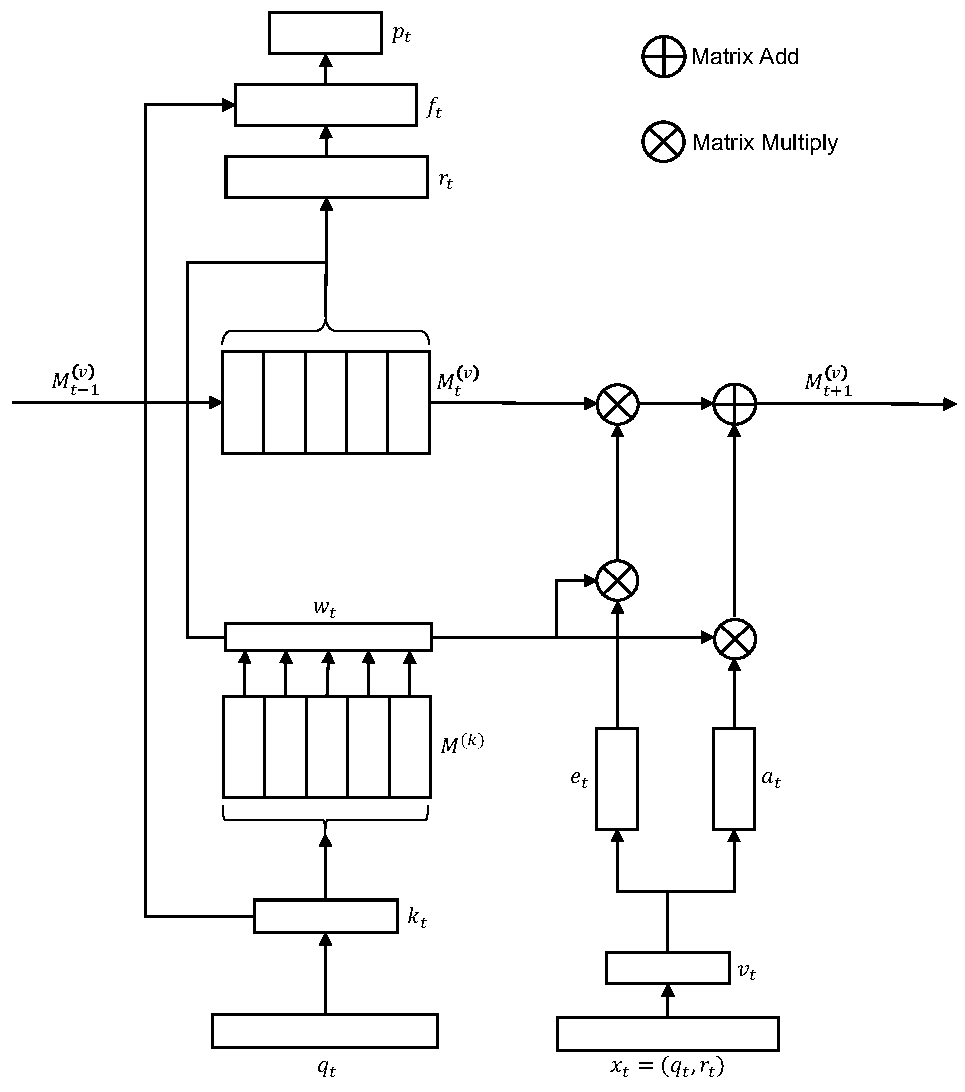
\includegraphics[width=0.9\textwidth]{ch3-dkvmn-model.pdf}
    \caption{The original dynamic key-value memory network model}\label{fig:ch3-dkvmn-model}
\end{figure}

In the reading process, the model weights and calculates the weight vector \(w_t\) with the knowledge point mastery matrix \(M^{(v)}\) to obtain the user's mastery representation vector \(r_t\) for the knowledge point. And \(r_t\) is spliced with the current exercise embedding vector \(k_t\), and \(f_t\) is derived after the full-linked activation layer loses \(Tanh(\cdot)\), which indicates the user's mastery of the exercise. The \(f_t\) goes through a final \(Sigmoid(\cdot)\) activation function to output a predicted probability of answering the exercise correctly \(p_t\). During the writing process, the current actual response performance will impact the student's knowledge acquisition status, which is a re-evaluation process. The current interaction record \(x_t=(q_t,a_t)\) will be used as the input to the model. Its embedding representation \(v_t\) will be used to compute the knowledge reduction vector \(e_t\) and the knowledge increase vector \(a_t\), and the reduction and increase vectors will be weighted with \(w_t\) and act on \(M^{(v)}\) thus realizing the change for the student's knowledge state. The training process is performed by minimizing the cross-entropy loss of \(p_t\) with the true label \(a_t\) of the correctness of the answers to the exercises. The whole model is microscopic and thus can be trained efficiently using stochastic gradient descent.

\section{Proposed Model}

\subsection{Algorithm Overview}
%本节的关键点是对学生的知识追踪,本文提出了一种针对DKVMN的改进型知识追踪网络模型,它在原模型的基础上增加了额外的用户答题特征,并通过图网络来改进知识点掌握度表征存储模块,从而为模型增加知识点间关系表征能力。本模型依然具有习题-知识点关联度计算、读取过程、写入过程和知识网络传播过程和预测过程等多个子模块。其模型框架如图。

The key point of this section is the knowledge tracing of students. In this thesis, an improved knowledge tracing network model for DKVMN was proposed, which adds additional user answer features to the original model and improves the knowledge point mastery representation storage module by graph networks, thus adding inter-knowledge point relationship representation capability to the model. The model still has several sub-modules such as exercise-knowledge point association degree calculation, reading process, writing process and knowledge network propagation process, and prediction process. Its model framework is shown in \figname{\ref{fig:ch3-gkvmn-model}}.

\begin{figure}[htbp!]
    \centering
    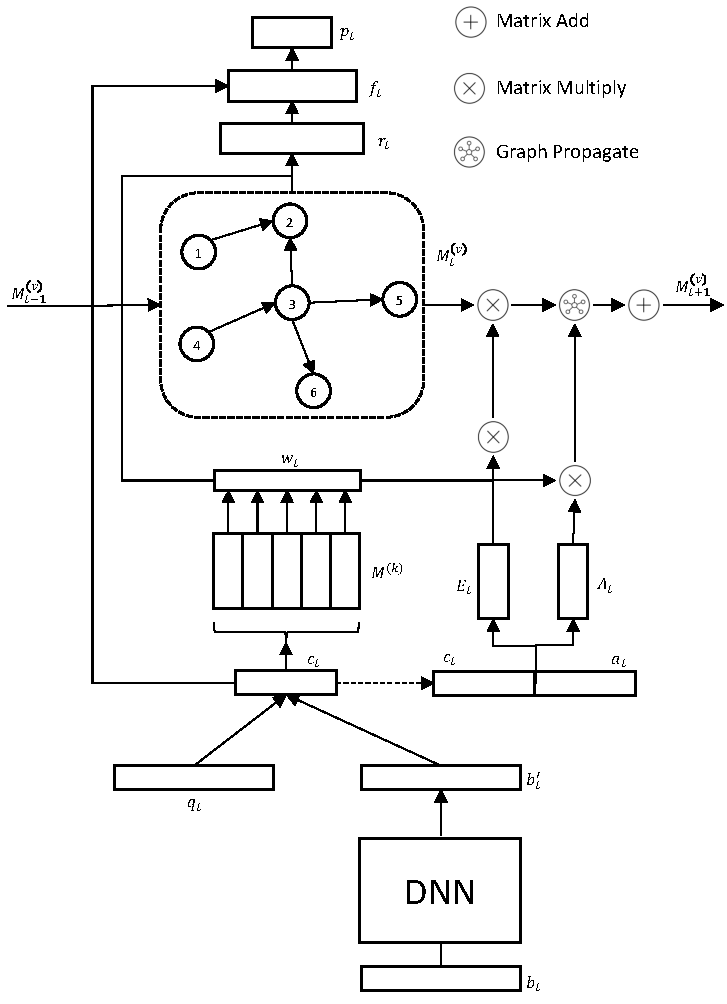
\includegraphics[width=0.9\textwidth]{ch3-gkvmn-model.pdf}
    \caption{The graph key-value memory network architecture}\label{fig:ch3-gkvmn-model}
\end{figure}

\subsection{Student Behavior Capturing}
%在本文中,提出了一种利用DNN来捕捉学生答题特征表征的机制,它与习题特征向量共同形成cross-feature向量,该向量用于后续的习题知识点权重向量计算,它将用户的答题行为特征(例如:是否hint、答题时间、尝试次数)向量\(b_1^t,b_2^t,\ldots,\b_N^t\)输入一个基于多层感知机的特征提取网络中,输出一个对于用户答题能力表征向量\(c_t\)。该向量与原始习题表示向量\(q_t\)进行特征交叉,生成融合用户特征的习题表征向量。具体过程如公式\eqname{\ref{fml:sbcap}}。

In this model, a mechanism is proposed to capture the student's answer feature representation using DNN, which together with the exercise feature vector forms the cross-feature vector that is used for the subsequent calculation of the exercise knowledge point weight vector, which takes the user's answer behavior features (e.g., whether hint, answer time, number of attempts) vector \(b_1^t,b_2^t,\ldots,b_N^t\) into a multilayer perceptron based feature extraction network and outputs a vector \(c_t\) for the user is answering ability representation. This vector is feature-crossed with the original exercise representation vector \(q_t\) to generate an exercise representation vector that incorporates user-related features. The specific process is shown in \eqname{\ref{fml:ch3-sbcap}}. The \(\| \) represents concatenation.

\begin{align}\label{fml:ch3-sbcap}
    \begin{split}
        b^{\prime}_t &= \operatorname{DNN}(b_1^t,b_2^t,\ldots,b_N^t) \\
        c_t &= q_t\|b^{\prime}_t
    \end{split}
\end{align}

%通过这种机制,模型引入了学生的个性化答题特征,从而可以实现对于习题知识点个性化权重计算。它充分利用了神经网络的特征表征能力,抽取出影响学生答题正确性的隐藏因素,从而提高模型整体的可靠性。
Through this mechanism, the model introduces students' personalized answering characteristics, thus enabling the calculation of personalized weights for the exercises' knowledge points. It makes full use of neural networks' feature characterization ability to extract the hidden factors that affect the correctness of students' answers, thus improving the overall reliability of the model.

\subsection{Knowledge-Question Correlation Calculation}
%在学生进行习题练习的过程中,一个习题与多个知识点相关,根据认知诊断理论\cite{chiu2018cognitive},学生对于知识点的掌握程度与学生的内在学习能力决定了学生答题的正确性。与DKVMN类似,本模型用Key矩阵\(M^{(k)}\)来保存习题相关的所有潜在知识点。假设共有\(N^{(K)}\)个知识点,则\(M^{(k)}\in\mathbb{R}^{N^{(K)}}\times d_k\),其中\(d_k\)为知识点表征向量的维度。

In the process of students' exercise practice, an exercise is associated with multiple knowledge points, and according to the cognitive diagnosis theory~\cite{chiu2018cognitive}, students' mastery of the knowledge points and students' intrinsic learning ability determine the correctness of their answers. Similar to DKVMN, this model uses the Key matrix \(M^{(k)}\) to keep all potential knowledge points related to the exercises. Suppose there are \(N^{(K)}\) knowledge points, then \(M^{(k)}\in\mathbb{R}^{{N^{(K)}}\times d_k}\), where \(d_k\) is the dimensionality of the knowledge point representation vector.

%在\eqname{\ref{fml:sbcap}}中,已经获取了融合学生个性化信息的习题表征向量\(c_t\),其中\(c_t\in\mathbb{R}^{d_k}\),对于第\(i\)个知识点概念,习题与知识点\(i\)的相关度\(w_t(i)\)的计算公式为\eqname{\ref{fml:ch3-corkq}},其中\(\sigma(\cdot)\)为softmax函数。

In \eqname{\ref{fml:ch3-sbcap}}, the exercise representation vector \(c_t\) incorporating students' personalized information has been obtained, where \(c_t\in\mathbb{R}^{d_k}\), and the correlation \(w_t(i)\) between the exercise and the knowledge point \(i\) for the \(i\)th knowledge point concept is calculated by is \eqname{\ref{fml:ch3-corkq}}, where \(\sigma(\cdot)\) is the softmax function.

\begin{align}\label{fml:ch3-corkq}
    \begin{split}
        w_t(i)=\sigma(c_t M^{(k)}(i))
    \end{split}
\end{align}

%由于\(M^{(k)}\)实际上是一个矩阵,因此可以通过矩阵运算来获得总体的相关向量\(\mathbf{w}_t=(w_t(1),w_t(2),\ldots,w_t(N^{(K)}))\)。
Since \(M^{(k)}\) is a matrix, the correlation vector \(\mathbf{w}_t=(w_t(1),w_t(2),\ldots,w_t(N^{(K)}))\) can be obtained by matrix operations like \eqname{\ref{fml:ch3-corkq-mat}}.

\begin{align}\label{fml:ch3-corkq-mat}
    \begin{split}
        \mathbf{w}_t=\sigma(c_t M^{(k)})
    \end{split}
\end{align}

%该向量代表习题与知识点的相关度表征,且经过融合用户的答题特征,能够捕获更多答题行为的影响因素。
The vector \(\mathbf{w}_t\) represents the relevance representation of the exercises and knowledge points, and after fusing the user's answer characteristics, it can capture more influencing factors of the answer behavior.

\subsection{Knowledge Mastery Calculation Process}
%本节的目的是计算用户对习题的潜在掌握程度,它是通过计算用户对习题相关知识点的掌握程度来完成。用户对于知识点的掌握程度通过一个矩阵\(M^{(v)}\in\mathbb{R}^{N^{(K)}\times d_v}\)来保存,其中\(d_v\)代表知识点掌握表征向量的维度。该矩阵与DKVMN的区别在于,矩阵会在后续经过图节点信息传播来对相关知识点进行掌握度修改。

The purpose of this section is to calculate the user's potential mastery of the exercise, which is performed by calculating the user's mastery of the knowledge points associated with the exercise. A matrix \ keeps the user's mastery of the knowledge points \((M^{(v)}\in\mathbb{R}^{N^{(K)}\times d_v}\), where \(d_v\) represents the dimensionality of the knowledge point mastery representation vector. The difference between this matrix and DKVMN is that the graph node information propagation will subsequently modify the matrix to the relevant knowledge points in terms of mastery.

%将前一节计算得到的习题与知识点的相关度表征向量\(\mathbf{w}_t\)与当前用户知识点掌握矩阵\(M^{(v)}\)进行加权和计算,如公式\eqname{\ref{}}所示
The correlation representation vector \(\mathbf{w}_t\) of the exercises and knowledge points calculated in the previous section is weighted and calculated with the current user knowledge mastery matrix \(M^{(v)}\), as shown in equation \eqname{\ref{fml:ch3-read}}.

\begin{align}\label{fml:ch3-read}
    \begin{split}
        r_t=\mathbf{w}_t M^{(v)}
    \end{split}
\end{align}

%计算得到的\(r_t\in\mathbb{R}^{d_v}\)表示用户对于习题的掌握程度,该向量考虑了用户的答题特征,相对于DKVMN融合了更多特征。本模型中,读取过程位于图传播计算之前,其目的在于防止图信息重复传播导致的信息增益爆炸。

In the model, the read process is located before the graph propagation calculation, and its purpose is to prevent the information gain explosion caused by repeated propagation of graph information.

\subsection{Knowledge Erase and Add Process with Graph Propagation}
%本节是计算用户在实际答题后,对于知识掌握的重新评估值。本节加入了图传播机制,它考虑了知识点的掌握程度变化引起的相关知识点的熟练度变化。本节的输入是\x_t=(c_t,a_t)\in\mathbb{R}^{(d_k+1)\times d_v}\),其中\(a_t\)是学生对于习题\(q_t\)的回答正确性嵌入表示,它与习题表征向量\(c_t\)共同用于计算答题记录嵌入表征向量\(v_t\),知识掌握增加向量\(A_t\)与知识掌握减少向量\(E_t\)。\(v_t\)的计算公式为\eqname{\ref{fml:ch3-write-vt}}. 
This section calculates the reassessment value of the user's knowledge mastery after actually answering the questions. This section incorporates a graph propagation mechanism, which takes into account the change in the proficiency of the relevant knowledge points caused by the change in the mastery of the knowledge points. The input of this section is \(x_t=(c_t,a_t)\in\mathbb{R}^{(d_k+1)\times d_v} \), where \(a_t\) is the embedded representation of the correctness of students' answers to the exercise \(q_t\), which is used together with the exercise representation vector \(c_t\) to compute the answer record embedding representation vector \(v_t\). the knowledge acquisition increase vector \(A_t\), and the knowledge acquisition decrease vector \(E_t\). The formula for \(v_t\) is \eqname{\ref{fml:ch3-write-vt}}.

\begin{align}\label{fml:ch3-write-vt}
    \begin{split}
        v_t &= \operatorname{Emb}(x_t)
    \end{split}
\end{align}

%知识掌握减少向量\(E_t\in\mathbb{R}^{d_v}\)通过\(v_t\)来计算,它被首先应用于知识掌握矩阵\(M^{(v)}\)。该计算通过加权和的方式完成。权重来自于前文计算得到的习题知识点相关矩阵\(\mathbf{w}_t\),对于第\(i\)个知识点知识掌握减少量\(\Delta{M^{(v)}(i)}_a\)和知识掌握增加量\(\Delta{M^{(v)}(i)}_e\)的计算公式是\eqname{\ref{fml:ch3-write-delta}}。其中\(W^{(e)}\in\mathbb{R}^{d_v \times d_v}\)和\(W^{(a)}\in\mathbb{R}^{d_v \times d_v}\)分别是\(E_t\)和\(A_t\)的转换矩阵,\(b^{(e)}\)和\(b^{(a)}\)分别为对应的偏置量。

The knowledge mastery reduction vector \(E_t\in\mathbb{R}^{d_v}\) is computed by \(v_t\), which is first applied to the knowledge mastery matrix \(M^{(v)}\). This calculation is done by means of a weighted sum. The weights are derived from the exercise knowledge point correlation matrix \(\mathbf{w}_t\) obtained from the previous calculation, and for the \(i\)th knowledge point knowledge mastery decrease \(\Delta_e{M^{(v)}(i)}\) and knowledge mastery increase \(\Delta_a{M^{(v)}(i)}\) are calculated as \eqname{\ref{fml:ch3-write-delta}}, where \(W^{(e)}\in\mathbb{R}^{d_v \times d_v}\) and \(W^{(a)}\in\mathbb{R}^{d_v \times d_v}\) are the transformation matrices of \(E_t\) and \(A_t\), respectively, and \(b^{(e)}\) and \(b^{(a)} \) are the corresponding biases, respectively.

\begin{align}\label{fml:ch3-write-delta}
    \begin{split}
        E_t &= \operatorname{Sigmoid}(W^{(e)}v_t+b^{(e)})\\
        A_t &= \operatorname{Tanh}(W^{(a)}v_t+b^{(a)})\\
        \Delta_e{M^{(v)}_t(i)} & = w_t(i) E_t \\
        \Delta_a{M^{(v)}_t(i)} & = w_t(i) A_t
    \end{split}
\end{align}

%在进行知识掌握熟练度更改时,先将原始的知识掌握向量的每个key slot与\(\Delta_e{M^{(v)}(i)}\)进行加权减法,然后加上知识掌握增益\Delta_a{M^{(v)}(i)} \如公式所示。

For the knowledge mastery proficiency change, each key slot of the original knowledge mastery vector is first weighted and subtracted from \(\Delta_e{M^{(v)}(i)}\), and then the knowledge mastery gain \(\Delta_a{M^{(v)}(i)}\) is added as shown in \eqname{\ref{fml:ch3-modify}}.

\begin{align}\label{fml:ch3-modify}
    \begin{split}
        \tilde{M^{(v)}_t}(i) &= M^{(v)}(i)(1-\Delta_e{M^{(v)}(i)}) \\
        \tilde{M^{(v)}_{t+1}}(i) &= \tilde{M^{(v)_t}}(i) + \Delta_a{M^{(v)}_t(i)}
    \end{split}
\end{align}

%最后,每个知识点的变化会对相邻知识点产生影响,因此此处引入了图网络传播机制,对整个知识掌握矩阵进行值重新分布。类似于图卷积神经网络的网络传播机制,则有公式\eqname{\ref{fml:ch3-graphpropagate}}。其中\(\tilde{M^{(v)}_{t+1}}(i))\in\mathbb{R}^{N^{(K)}\times d_v}\)为图网络的上一层和输入。\(M^{(v)}_{t+1}(i)\)为图网络的下一层。\(\tilde{A}=A+I_{N^{(K)}}\)为自连接邻接矩阵。\(\tilde{D}\)为度矩阵,即\(\tilde{D}_ii=\sum_j{\tilde{A}_ij}\),\(W_t\in\mathbb{R}^{d_v \times d_v}\)为待训练的权重矩阵。\(\sigma(\cdot)\)为激活函数,在此处使用\(LeakyReLU(\cdot)\)。

Finally, changes in each knowledge point have an impact on neighboring knowledge points, so a graph network propagation mechanism is introduced here to redistribute the values across the knowledge mastery matrix. Similar to the network propagation mechanism of graph convolutional neural network, then there is the formula \eqname{\ref{fml:ch3-graphpropagate}}, where \(\tilde{M^{(v)}_{t+1}}(i)\in\mathbb{R}^{N^{(K)}\times d_v}\) is the upper layer of the graph network and the input. \(M^{(v)}_{t+1}(i)\) is the next layer of the graph network. \(\tilde{A}=A+I_{N^{(K)}}\) is the self-connected adjacency matrix. \(\tilde{D}\) is the degree matrix, i.e. \(\tilde{D}_{ii}=\sum_j{\tilde{A}_{ij}}\), \(W_t\in\mathbb{R}^{d_v \times d_v}\) is the matrix of weights to be trained. \(\sigma(\cdot)\) is the activation function, and \(LeakyReLU(\cdot)\) is used here.

\begin{align}\label{fml:ch3-graphpropagate}
    M^{(v)}_{t+1}(i) \leftarrow \sigma(\tilde{D}^{-\frac{1}{2}}\tilde{A}\tilde{D}^{\frac{1}{2}}\tilde{M^{(v)}_{t+1}}(i)W_t)
\end{align}

%由此可见,知识点的邻接矩阵是图传播的关键,本文提出了基于统计的方式来计算知识点邻接矩阵\(A\),即当知识点\(i,j\)共现次数超过某一阈值时,将\(i,j\)知识点设置为相关。如公式\eqname{\ref{fml:ch3-confidence}}所示。

It can be seen that the adjacency matrix of knowledge points is the key to graph propagation, and this thesis proposes a statistical-based approach to calculate the knowledge point adjacency matrix \(A\), i.e., when the number of co-occurrences of knowledge points \(i,j\) exceeds a certain threshold, \(i,j\) knowledge points are set to be relevant. As shown in equation \eqname{\ref{fml:ch3-confidence}}, the \(P_{ij}\) represents the probability that exercise \(i\) and exercise \(j\) exist in one exercise.
\begin{align}\label{fml:ch3-confidence}
    A_{ij}=\{\begin{array}{ll}
        0, & \text{ if } P_{ij}<\tau^{(k)}      \\
        1, & \text{ if } P_{ij} \geq \tau^{(k)}
    \end{array}
\end{align}


Finally, changes in each knowledge point have an impact on neighboring knowledge points, so a graph network propagation mechanism is introduced here to redistribute the values across the knowledge mastery matrix.


% \subsubsection{Statistics-based Method}


% \subsubsection{Multi-head Attention Based}


\subsection{Prediction}
%经过计算得到的知识点掌握熟练度表征\(r_t\)可以用于计算习题回答正确的概率。它通过中间和向量\(f_t\)来计算,其中\(f_t\)包含了习题相关知识点的掌握程度和习题本身的信息。计算公式如\eqname{\ref{fml:ch3-predicting-function-f}}}所示,其中权重转移矩阵\(W_f\)和偏置向量\(b_f\)为待训练参数。
The computed knowledge point mastery proficiency representation \(r_t\) can be used to calculate the probability of answering the exercise correctly. It is calculated by the intermediate sum vector \(f_t\), where \(f_t\) contains information about the mastery of the knowledge points related to the exercise and the exercise itself. The calculation formula is shown in \eqname{\ref{fml:ch3-predicting-function-f}}, where the weight transfer matrix \(W_f\) and the bias vector \(b_f\) are the parameters to be trained.
\begin{align}\label{fml:ch3-predicting-function-f}
    f_t = \operatorname{Tanh}(W_f^T[r_t,c_t] + b_f)
\end{align}

%然后经过一个全连接激活层,输出对于习题\(q_t\)的正确性预测\(p_t\)。计算公式如\eqname{\ref{fml:ch3-predicting-function-p}},其中权重转移矩阵\(W_p\)和偏置向量\(b_p\)为待训练参数。
Then after a fully connected activation layer, the correctness prediction \(p_t\) for the exercise \(q_t\) is output. The formula is calculated as \eqname{\ref{fml:ch3-predicting-function-p}}, where the weight transfer matrix \(W_p\) and the bias vector \(b_p\) are the parameters to be trained.
\begin{align}\label{fml:ch3-predicting-function-p}
    p_t = \operatorname{Sigmoid}(W_p^T f_t + b_p)
\end{align}

%整个网络通过端到端的训练来进行,真实的正确性为\(a_t\),整体的损失函数为
The whole network is trained in an end-to-end manner j with true correctness \(a_t\), and the overall loss function is \eqname{\ref{fml:ch3-loss}}.
\begin{align}\label{fml:ch3-loss}
    \mathcal{L} = -\sum\limits_{t}{(a_t\log(p_t)+(1-a_t)\log(1-p_t))}
\end{align}


\subsection{Knowledge Mastery}
Due to the nature of GKVMN, the knowledge mastery \(M^{(v)}\) is explicit so that it can be directly used as a kind of recommendation system for judgment. Moreover, it can be subsequently used as a student knowledge mastery state analysis.

\section{Experiments}
%本节中,通过多个专用的知识追踪数据集来investigate提出的模型性能,与目前已经提出的Baseline模型进行性能对比。本章先对所用到的数据集进行介绍和统计,然后提出用于模型性能对比的度量标准、实验设置和运行参数环境等,最后得出结果并进行分析。
In this section, algorithms, including the performance, are investigated through multiple dedicated knowledge tracing data sets, and the performance of the proposed baseline model is compared. This chapter first introduces and counts the data sets used, then proposes metrics, experimental settings, and operating parameter environments for model performance comparison, and finally draws the results and analyzes them.

\subsection{Datasets}
After investigating the existing knowledge tracing model, the thesis selected the more popular ASSISTment data set and Statics data set related to mathematics, preprocessed the data set, cleaned the data, obtained the training set, and performed the performance with the Baseline model Compared.
%本实验主要采用ASSISTment2009数据集用于测试,该数据集是在2009-2010学年于ASSISTment教学平台上采集的真实教育数据。该数据集包含一个Skill builder问题集合,当学生达到一定的标准时,即被认为是掌握了某个技能。当学生掌握某个技能后,将不会有关于该技能的习题推送。

The experiment was conducted using the ASSISTment 2009 dataset, which is a collection of real educational data collected on the ASSISTment teaching platform during the 2009-2010 academic year. The dataset contains a set of Skill builder questions, where students are considered to have mastered a skill when they meet specific criteria. Once a student has mastered a skill, there will be no exercises pushed for that skill.


\subsubsection{Data Description}
%在该数据集的基础记录中,每一行为一个问题的答题记录,包含一系列的特征,例如问题的Id表示problem_id,学生的ID表示user_id,学生的答题次数attempt_count,学生答题用时ms_first_response,问题的相关技能ID表示skill_id等,具体的描述如下:

In the base record of this dataset, each row is a question answering record, containing a series of features, such as problem\_id, user\_id, attempt\_count, ms\_first\_response skill\_id, etc. The specific description is as \tblname{\ref{tbl:ch3-assist2009-heading}}.

\begin{table}[htbp!]
    \centering
    \caption{The column heading of ASSISTment Dataset}\label{tbl:ch3-assist2009-heading}
    \begin{tabular}{lc}
        \toprule
        column heading & description                                                       \\
        \midrule
        problem\_id    & problem or exercise ID                                            \\
        user\_id       & the ID of the user                                                \\
        correct        & a binary value, 1 represents correct while 0 represents incorrect \\
        attempt\_count & Number of student attempts on the exercise                        \\
        skill\_id      & skill ID associated with the exercise                             \\
        hint\_count    & Number of student attempts on this problem                        \\
        first\_action  & The Whether or not the student asks for all hints                 \\
        \bottomrule
    \end{tabular}
\end{table}

%经过统计,数据集的一些基本统计数据如下
The statistical information of the dataset ASSISTment 2009 after data pre-processing is shown in the \tblname{\ref{tbl:ch3-assist2009-stat}}.
\begin{table}
    \centering
    \caption{Statistics of ASSISTment 2009 dataset}\label{tbl:ch3-assist2009-stat}
    \begin{tabular}{ccccc}
        \toprule
        Statistics      & \makecell[c]{Number                          \\ of Students} & \makecell[c]{Number                         \\of Skills }& \makecell[c]{Number                         \\of Questions }& \makecell[c]{Number                         \\ of Records} \\
        \midrule
        ASSISTment 2009 & 4,032               & 124 & 17,748 & 459,092 \\
        \bottomrule
    \end{tabular}
\end{table}
% Total number of students: 4032
% Training set size: 2580
% Validation set size: 645
% Testing set size: 806
% Number of skills: 123
% Number of features in the input: 246

\subsubsection{Data Preprocessing}
%数据预处理是进行模型训练的重要前置步骤。在原始数据中,部分关键的特征出现了缺失,因此应当首先进行数据清洗,清除这些行。例如:缺失关键的skill\_id,correctness和user\_id的行会被剔除。由于知识追踪等任务是基于个体层面进行,因此一个知识追踪的输入序列必须属于同一个用户。而在原始数据集中,这样的序列是乱序的,因此需要对用户的答题序列基于用户个体做聚合排序处理。为了将答题的正确性融入到特征,需要进行特征交叉,在此处的特征交叉是将skill_id与correct两个特征进行加权相加和平移来进行。特征交叉可以为模型带来非线性。
Data preprocessing is an important antecedent step to perform model training. Some key features are missing in the raw dataset, so data cleaning should be performed first to remove these rows. For example, rows missing the key skill\_id, correctness, and user\_id will be excluded. Since knowledge tracing is performed on an individual level, the input sequence of knowledge tracing must belong to the same user. In the original dataset, such sequences are disordered, so it is necessary to perform aggregated sorting of the user's answer sequences based on individual users. In order to incorporate the correctness of the answers into the new features, feature crossover is required, where the feature crossover is performed by weighting the two features, skill\_id and correct, by summing and translating them. Feature crossing can introduce nonlinearity into the model.
% \begin{itemize}
%     \item problem\_id: problem or exercise ID.\
%     \item user\_id: the ID of the user.
%     \item correct: a binary value, 1 represents correct while 0 represents incorrect.
%     \item attempt_count:
% \end{itemize}

%本实验设置了最长训练序列长度作为超参数,因此对于超过最长训练序列的输入序列,需要进行分割。
In this experiment, the length of the longest training sequence is set as the hyperparameter, so for the input sequence that exceeds the longest training sequence, segmentation is required.
%(1)ASSISTment 2015 是一个用于预测学生考试表现的数据集,它由一系列包含若干知识点标签的问题以及一些学生的答题记录组成。它在2015年于线上教育平台上采集而成。经过数据过滤获得包含19917个学生,约102千个问题,100个知识点标签和约709次交互的数据集。
%(2)ASSISTment 2017 来源于2017年举办的ASSISTments Longitudinal Data Mining Competition。经过数据预处理和数据过滤,数据集包含1709个学生,4117个问题,102个知识点和约943千次交互。
%(3)Statics 2011 数据集来源于统计学课程的答题记录。

\subsubsection{Data Analysis}
%在进行模型训练之前,针对数据集进行因果分析,来筛选出合理的变量作为模型输入可以有效提高模型性能。在本节,从经过预处理的原始数据,选取出可能对最终产生影响的若干特征,进行可视化分析。然后选择合适的特征进行输入。
Before model training, a dependent variable analysis is performed for the dataset to filter out reasonable variables as model inputs can effectively improve model performance. In this section, several features that may impact the final are selected for visualization and analysis from the preprocessed raw data. The appropriate features are then selected for input.
%首先,可以对原数据源进行列相关度分析,获取各个输入特征与输出结果标签的相关度。绘制的列相关度热力图如图所示。可见是与习题答题正确性最相关的几个特征。因此本实验将这些特征作为用户的行为特征加入模型。
First, column correlation analysis can be performed on the original data source to obtain each input feature's correlation with the output result labels. The plotted column correlation heat map is shown in \figname{\ref{fig:ch3-dataset-heatmap}}.

\begin{figure}[htb]
    \centering
    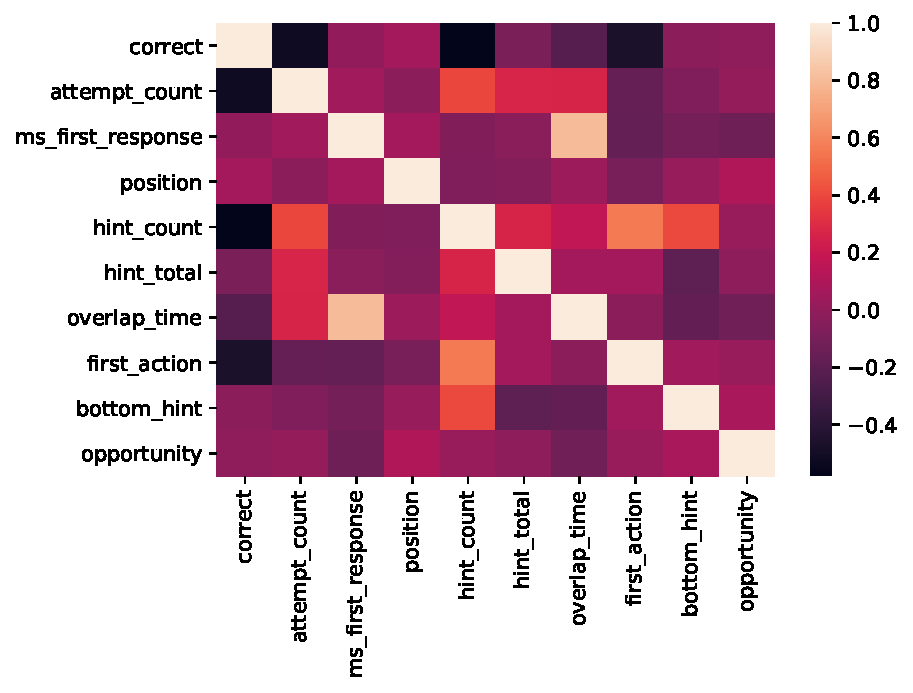
\includegraphics[width=0.85\textwidth]{ch3-dataset-heatmap.pdf}
    \caption{The heat map of original dataset ASSISTment 2009}\label{fig:ch3-dataset-heatmap}
\end{figure}

%然后,结合热力图,分别对筛选出来的特征绘制互相关性图与分布图,得到. 由此可见,这些特征存在一定的互相关性。
Then, combined with the heat map, the mutual correlation map and distribution map are plotted for the filtered features, respectively. The figure is \figname{\ref{fig:ch3-dataset-corrplot}}. It can be seen that there is a certain mutual correlation of these features.
\begin{figure}[htbp!]
    \centering
    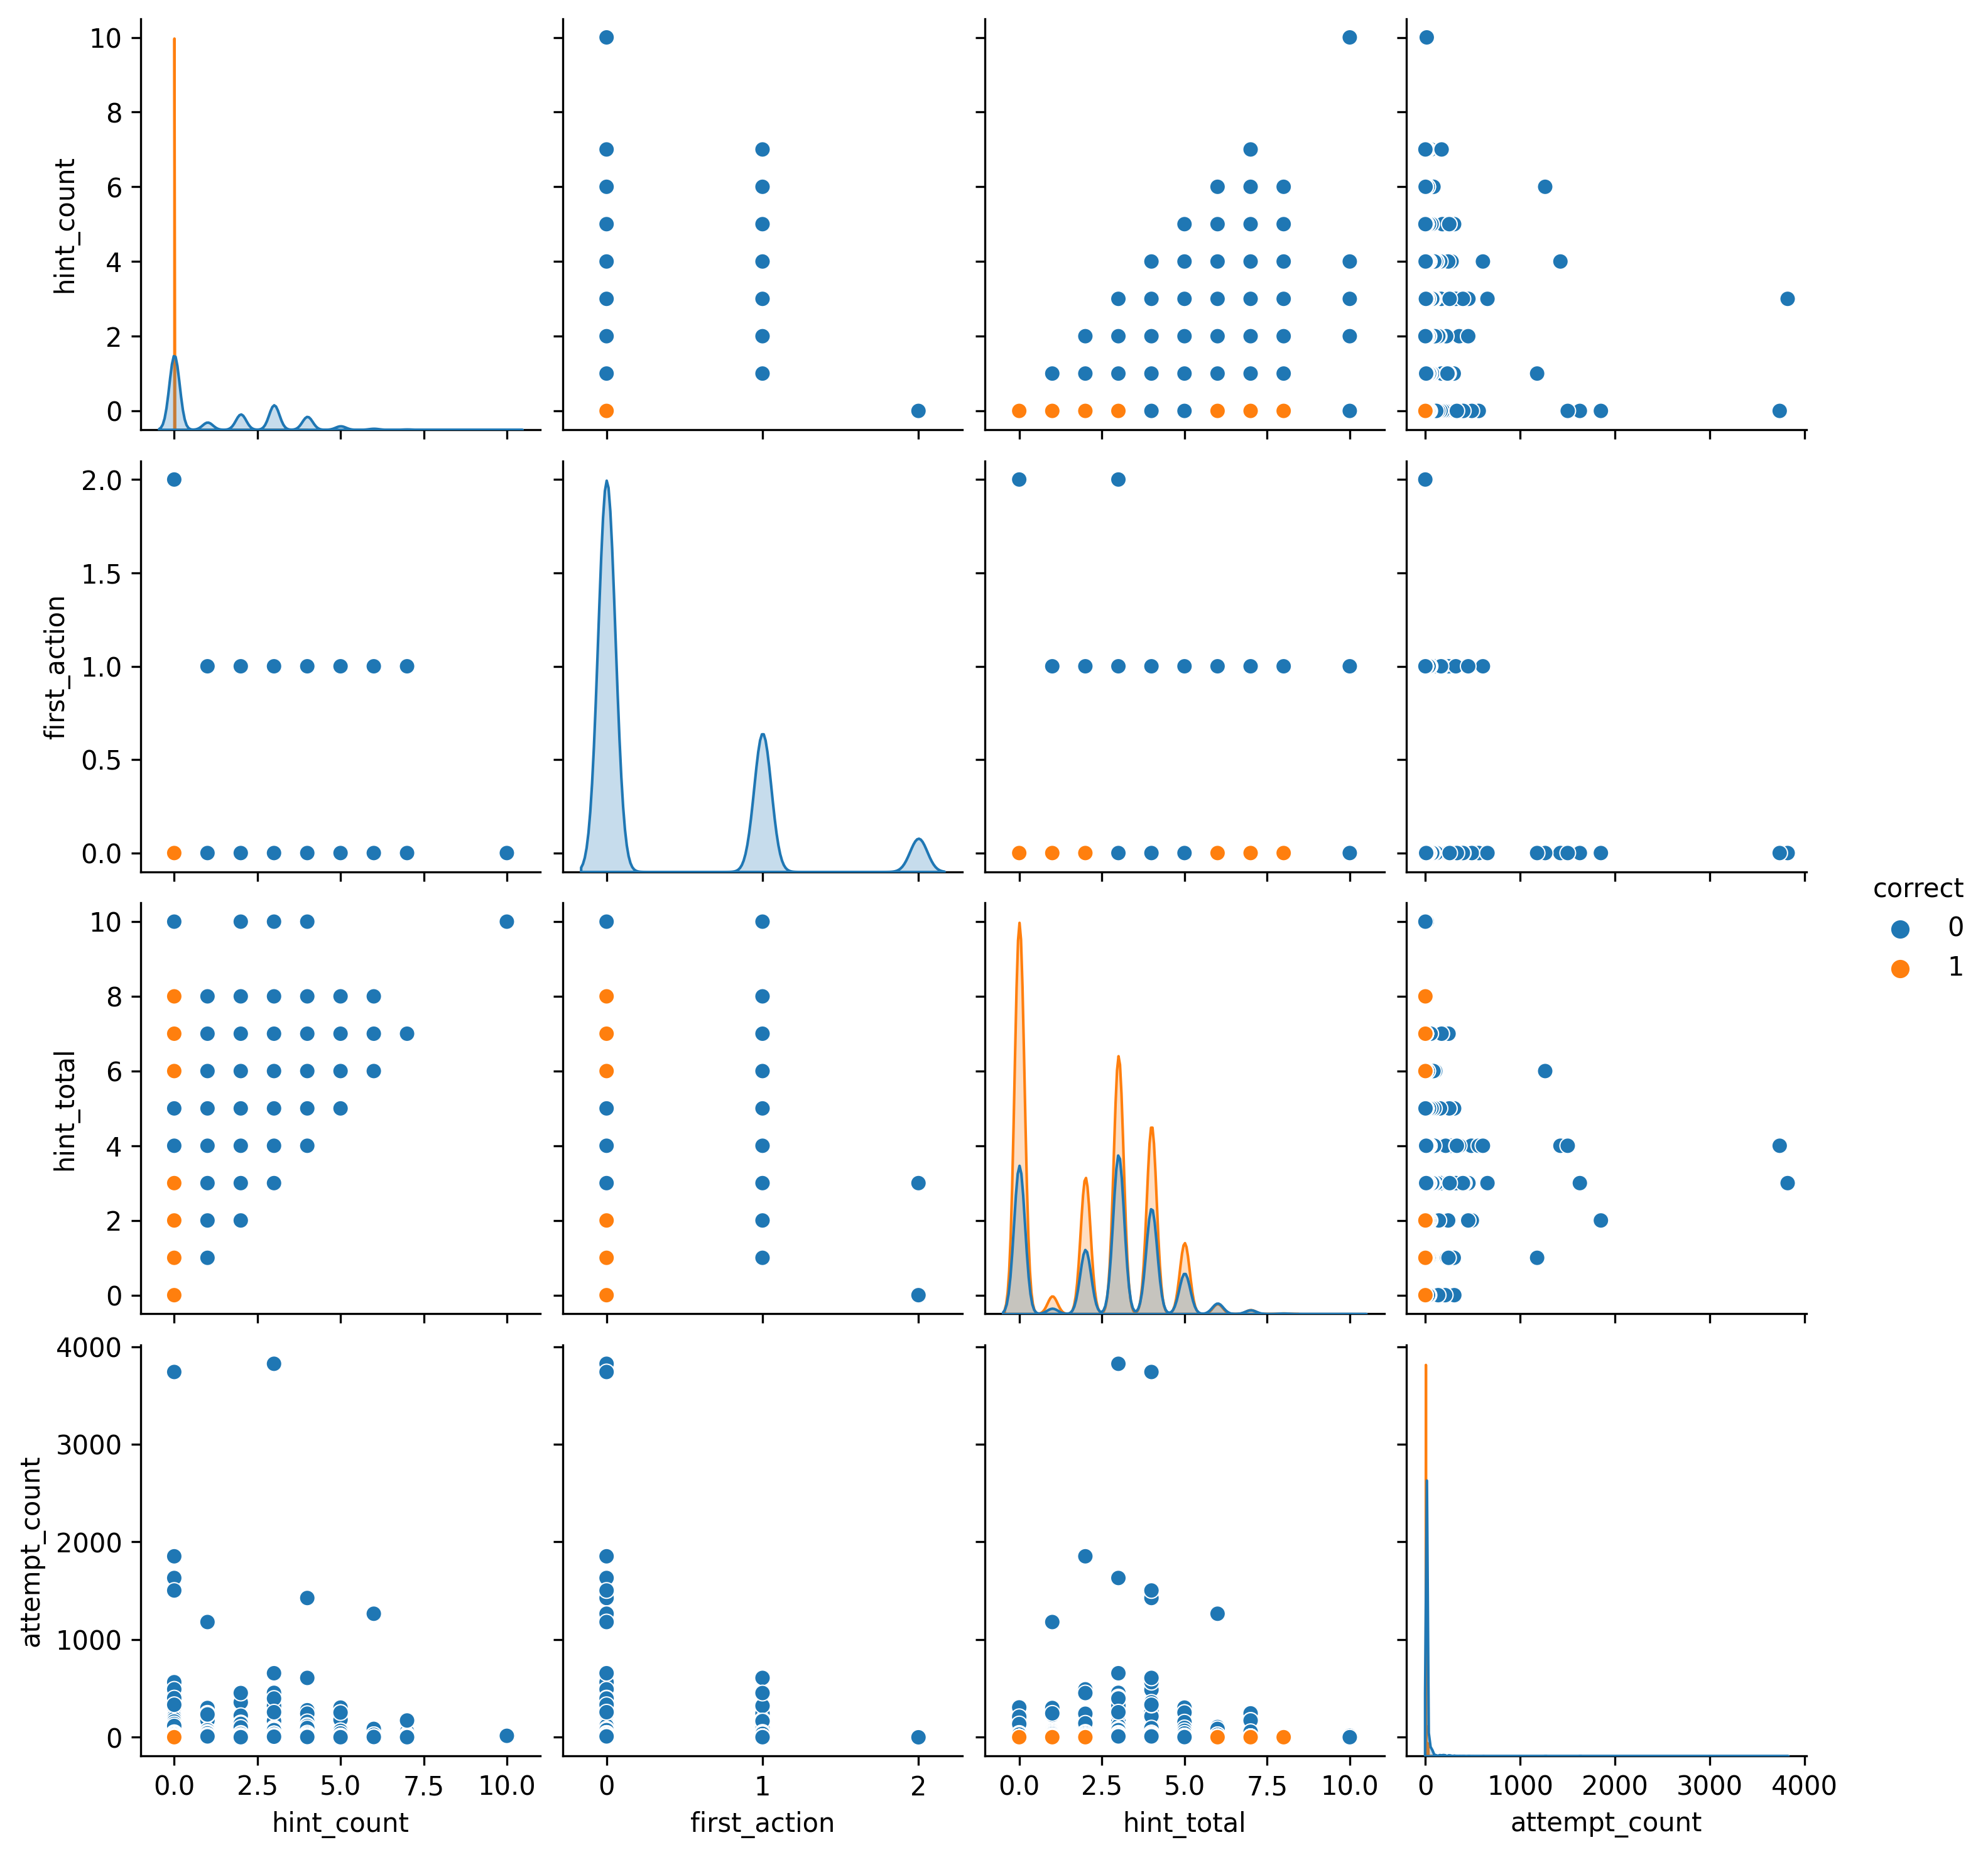
\includegraphics[width=1.0\textwidth]{ch3-dataset-corrplot.png}
    \caption{The correlation plot between features and correctness}\label{fig:ch3-dataset-corrplot}
\end{figure}


%接下来,将每个特征与答题正确性分别绘制互相关图,分析各个特征与目标特征的关系。
Next, each feature was plotted separately against the correctness of the answer, and the relationship between each feature and the target feature was analyzed, as shown in \figname{\ref{fig:ch3-jointplots}}.
\begin{figure}[htbp!]
    \centering
    \begin{subfigure}[b]{0.475\textwidth}
        \centering
        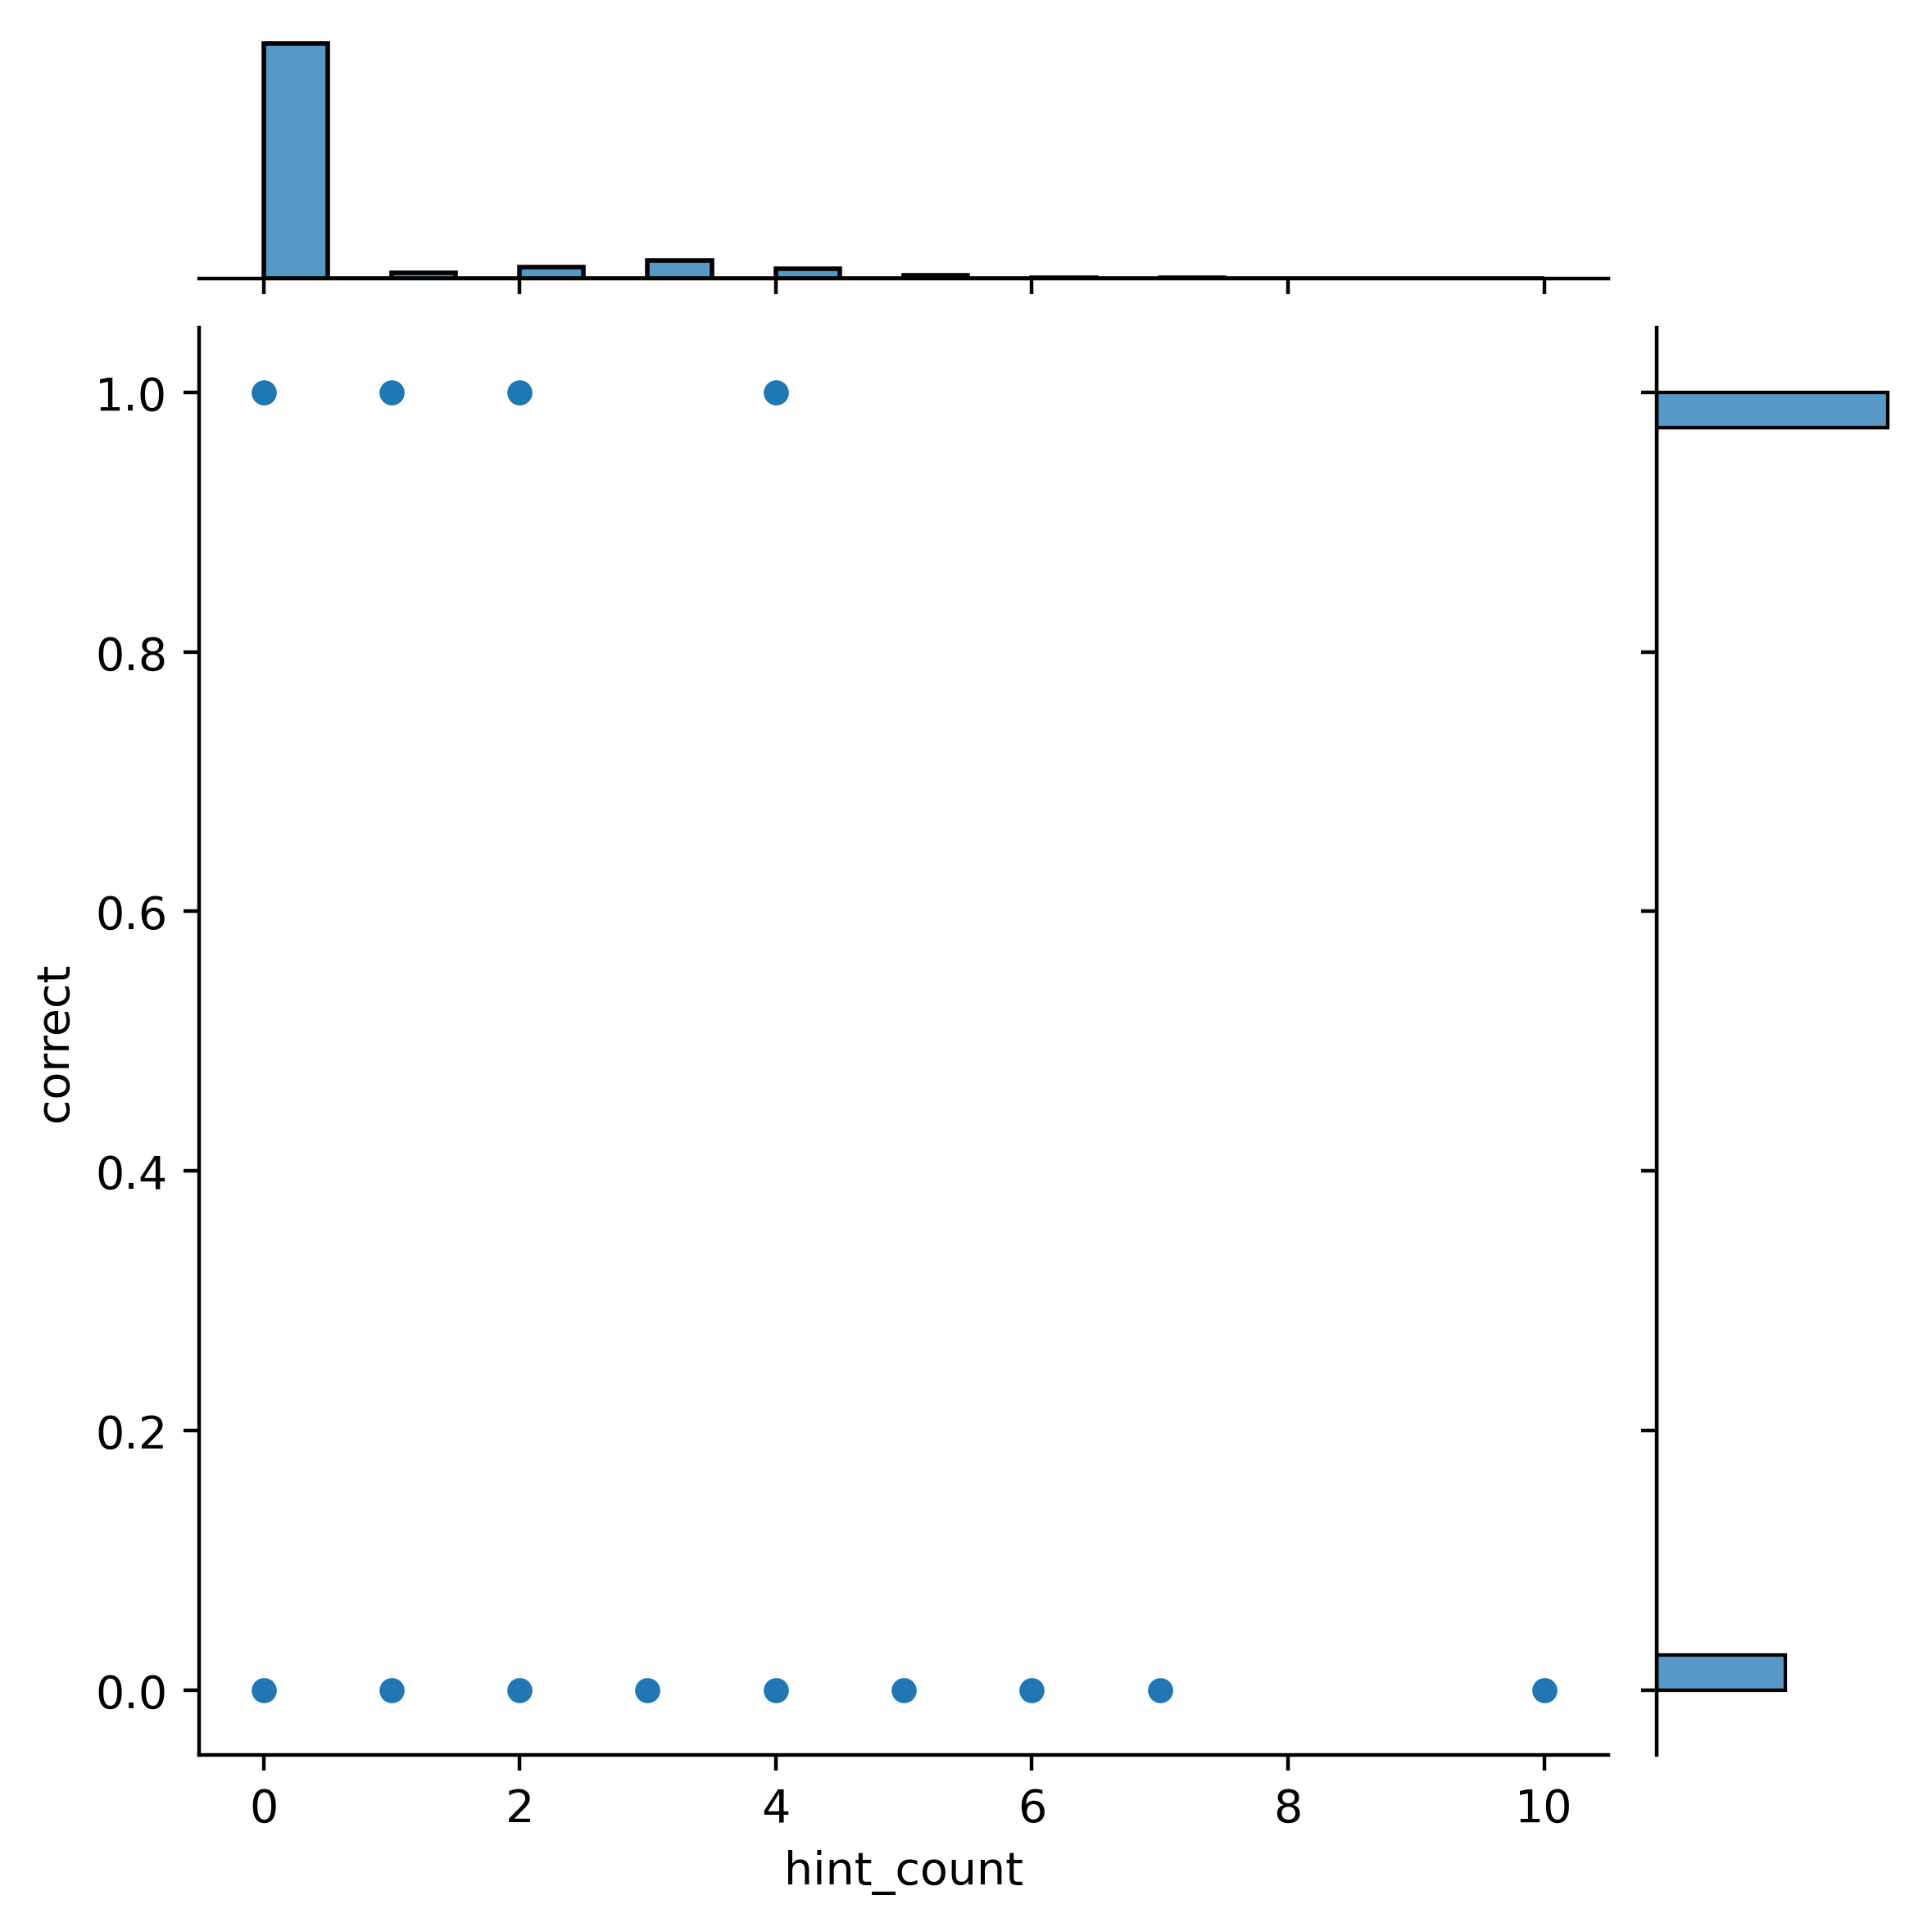
\includegraphics[width=0.9\textwidth]{ch3-jointplot-hc.png}
        \caption[dis]{The joint-plot of hint\_count}\label{fig:ch3-jointplot-hc}
    \end{subfigure}
    \begin{subfigure}[b]{0.475\textwidth}
        \centering
        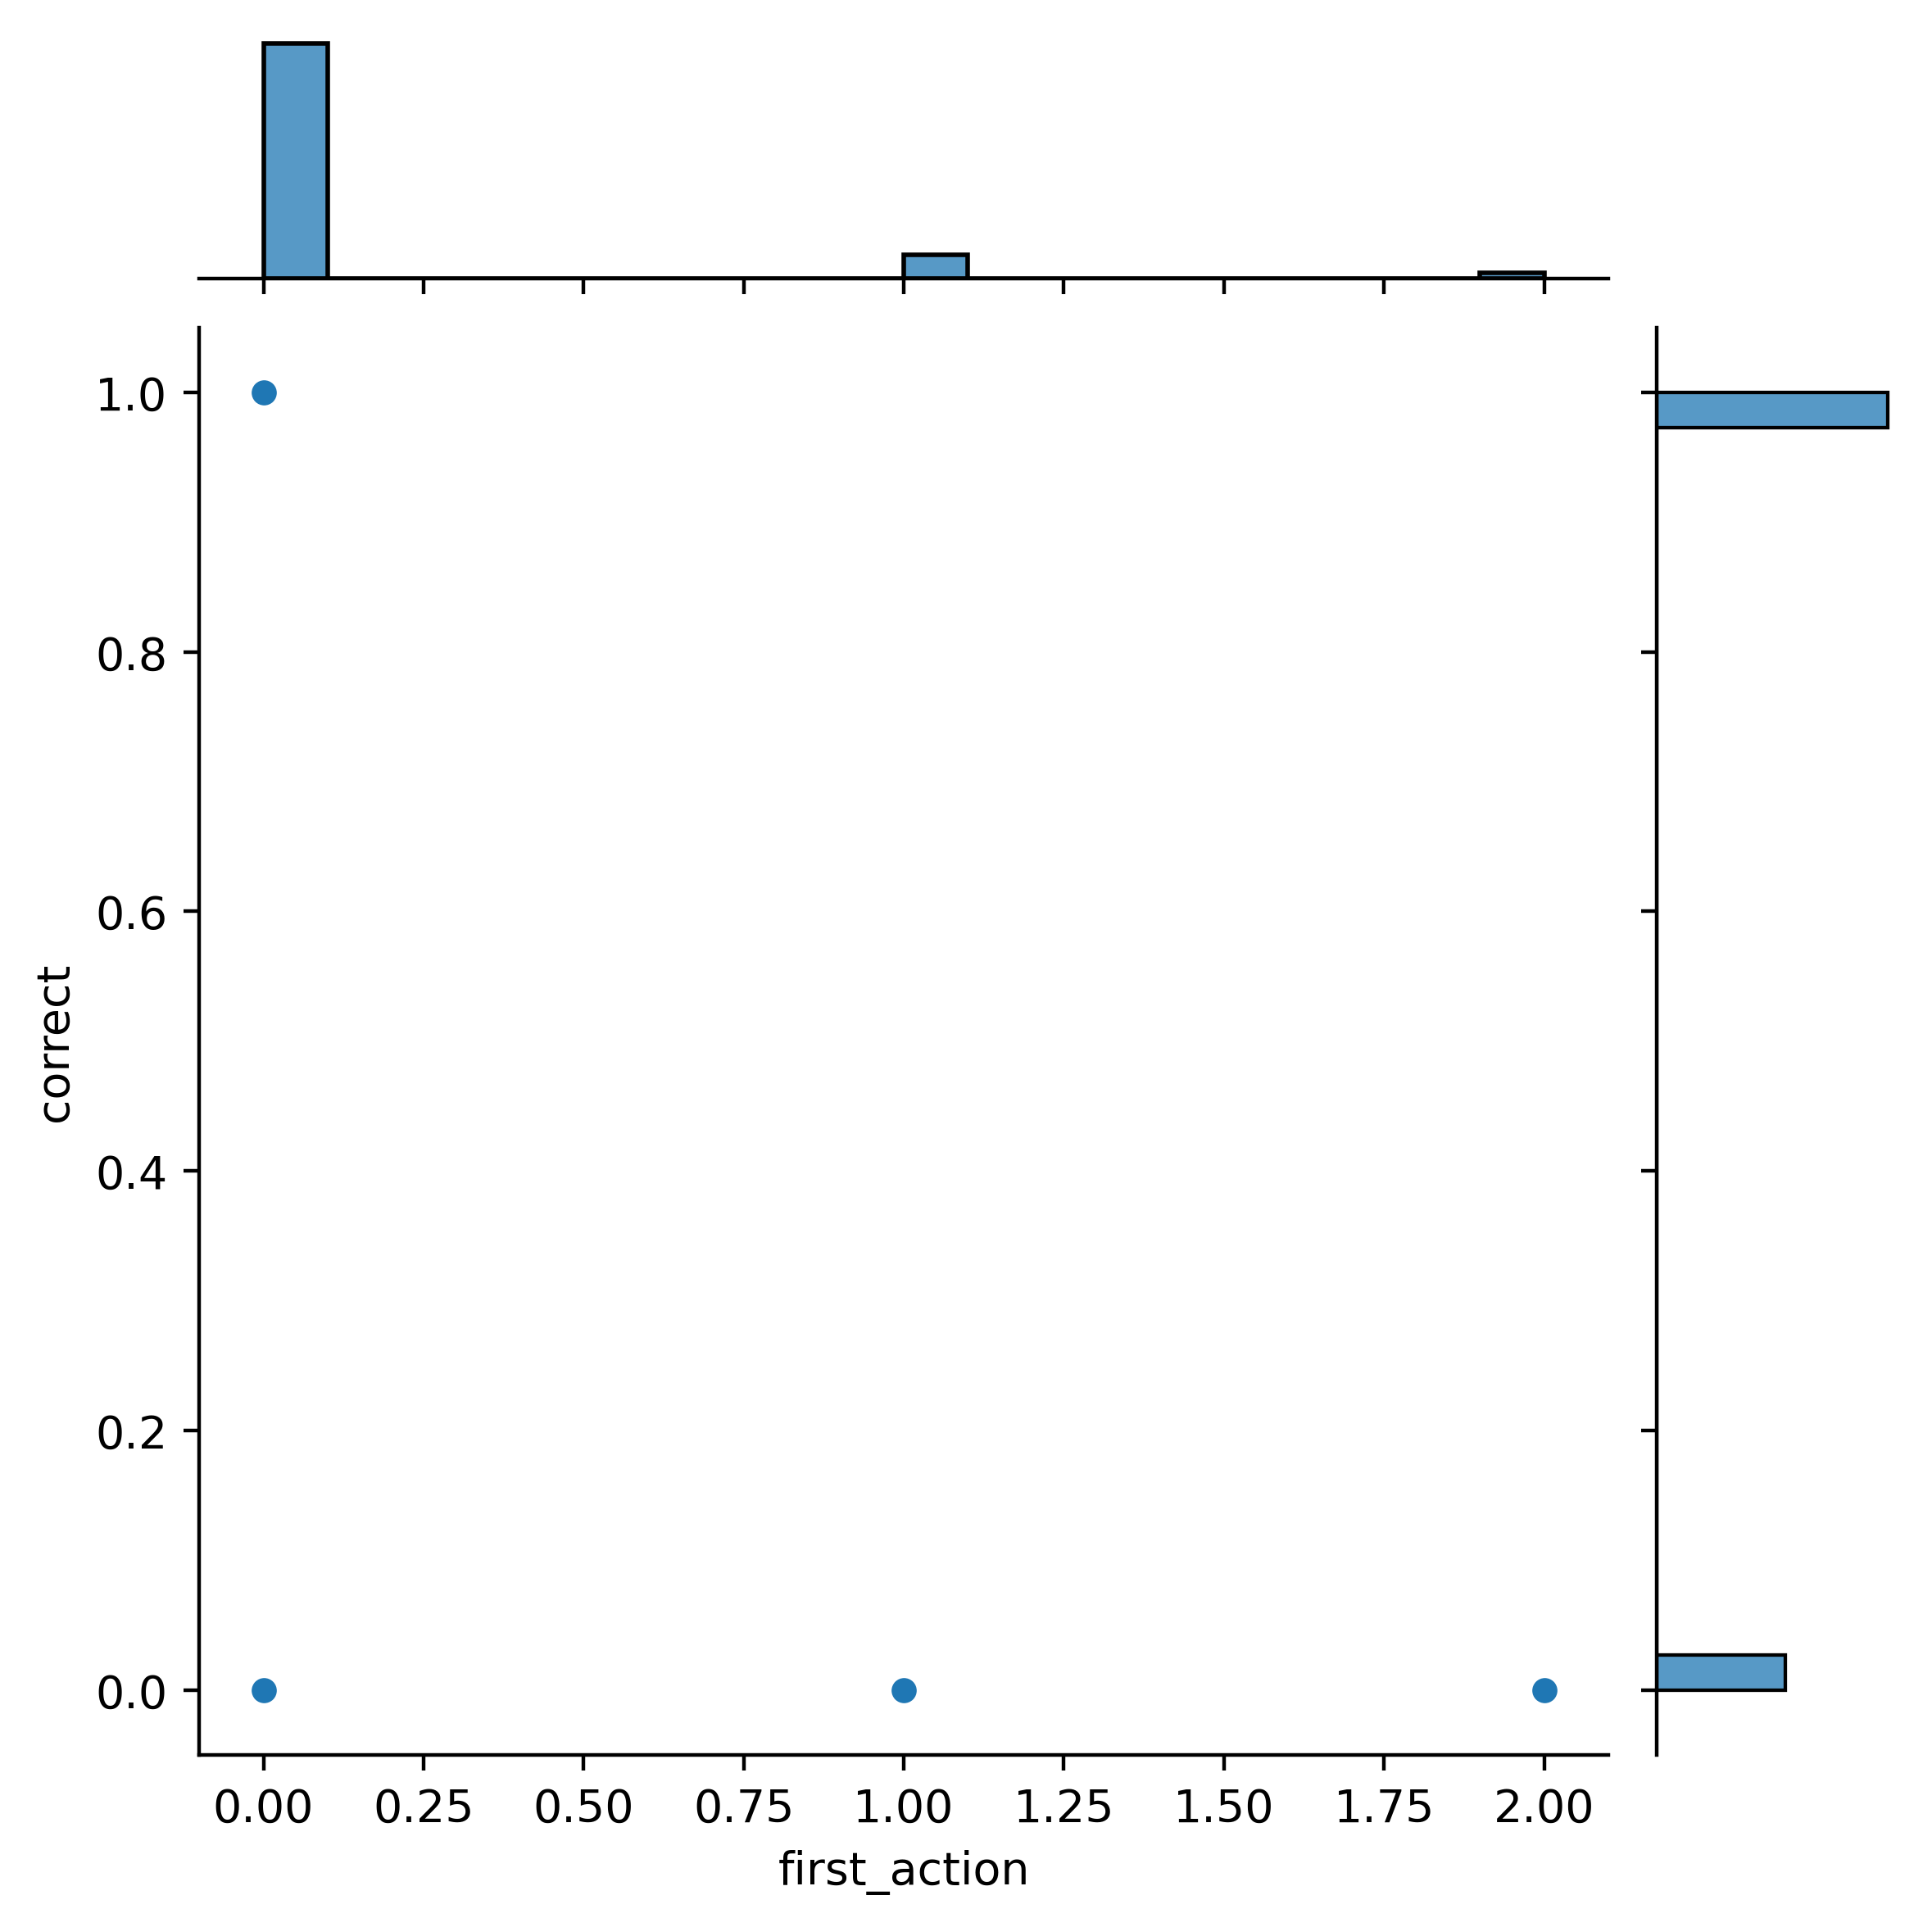
\includegraphics[width=0.9\textwidth]{ch3-jointplot-fc.png}
        \caption{The joint-plot of first\_action}\label{fig:ch3-jointplot-fc}
    \end{subfigure}
    \\
    \begin{subfigure}[b]{0.475\textwidth}
        \centering
        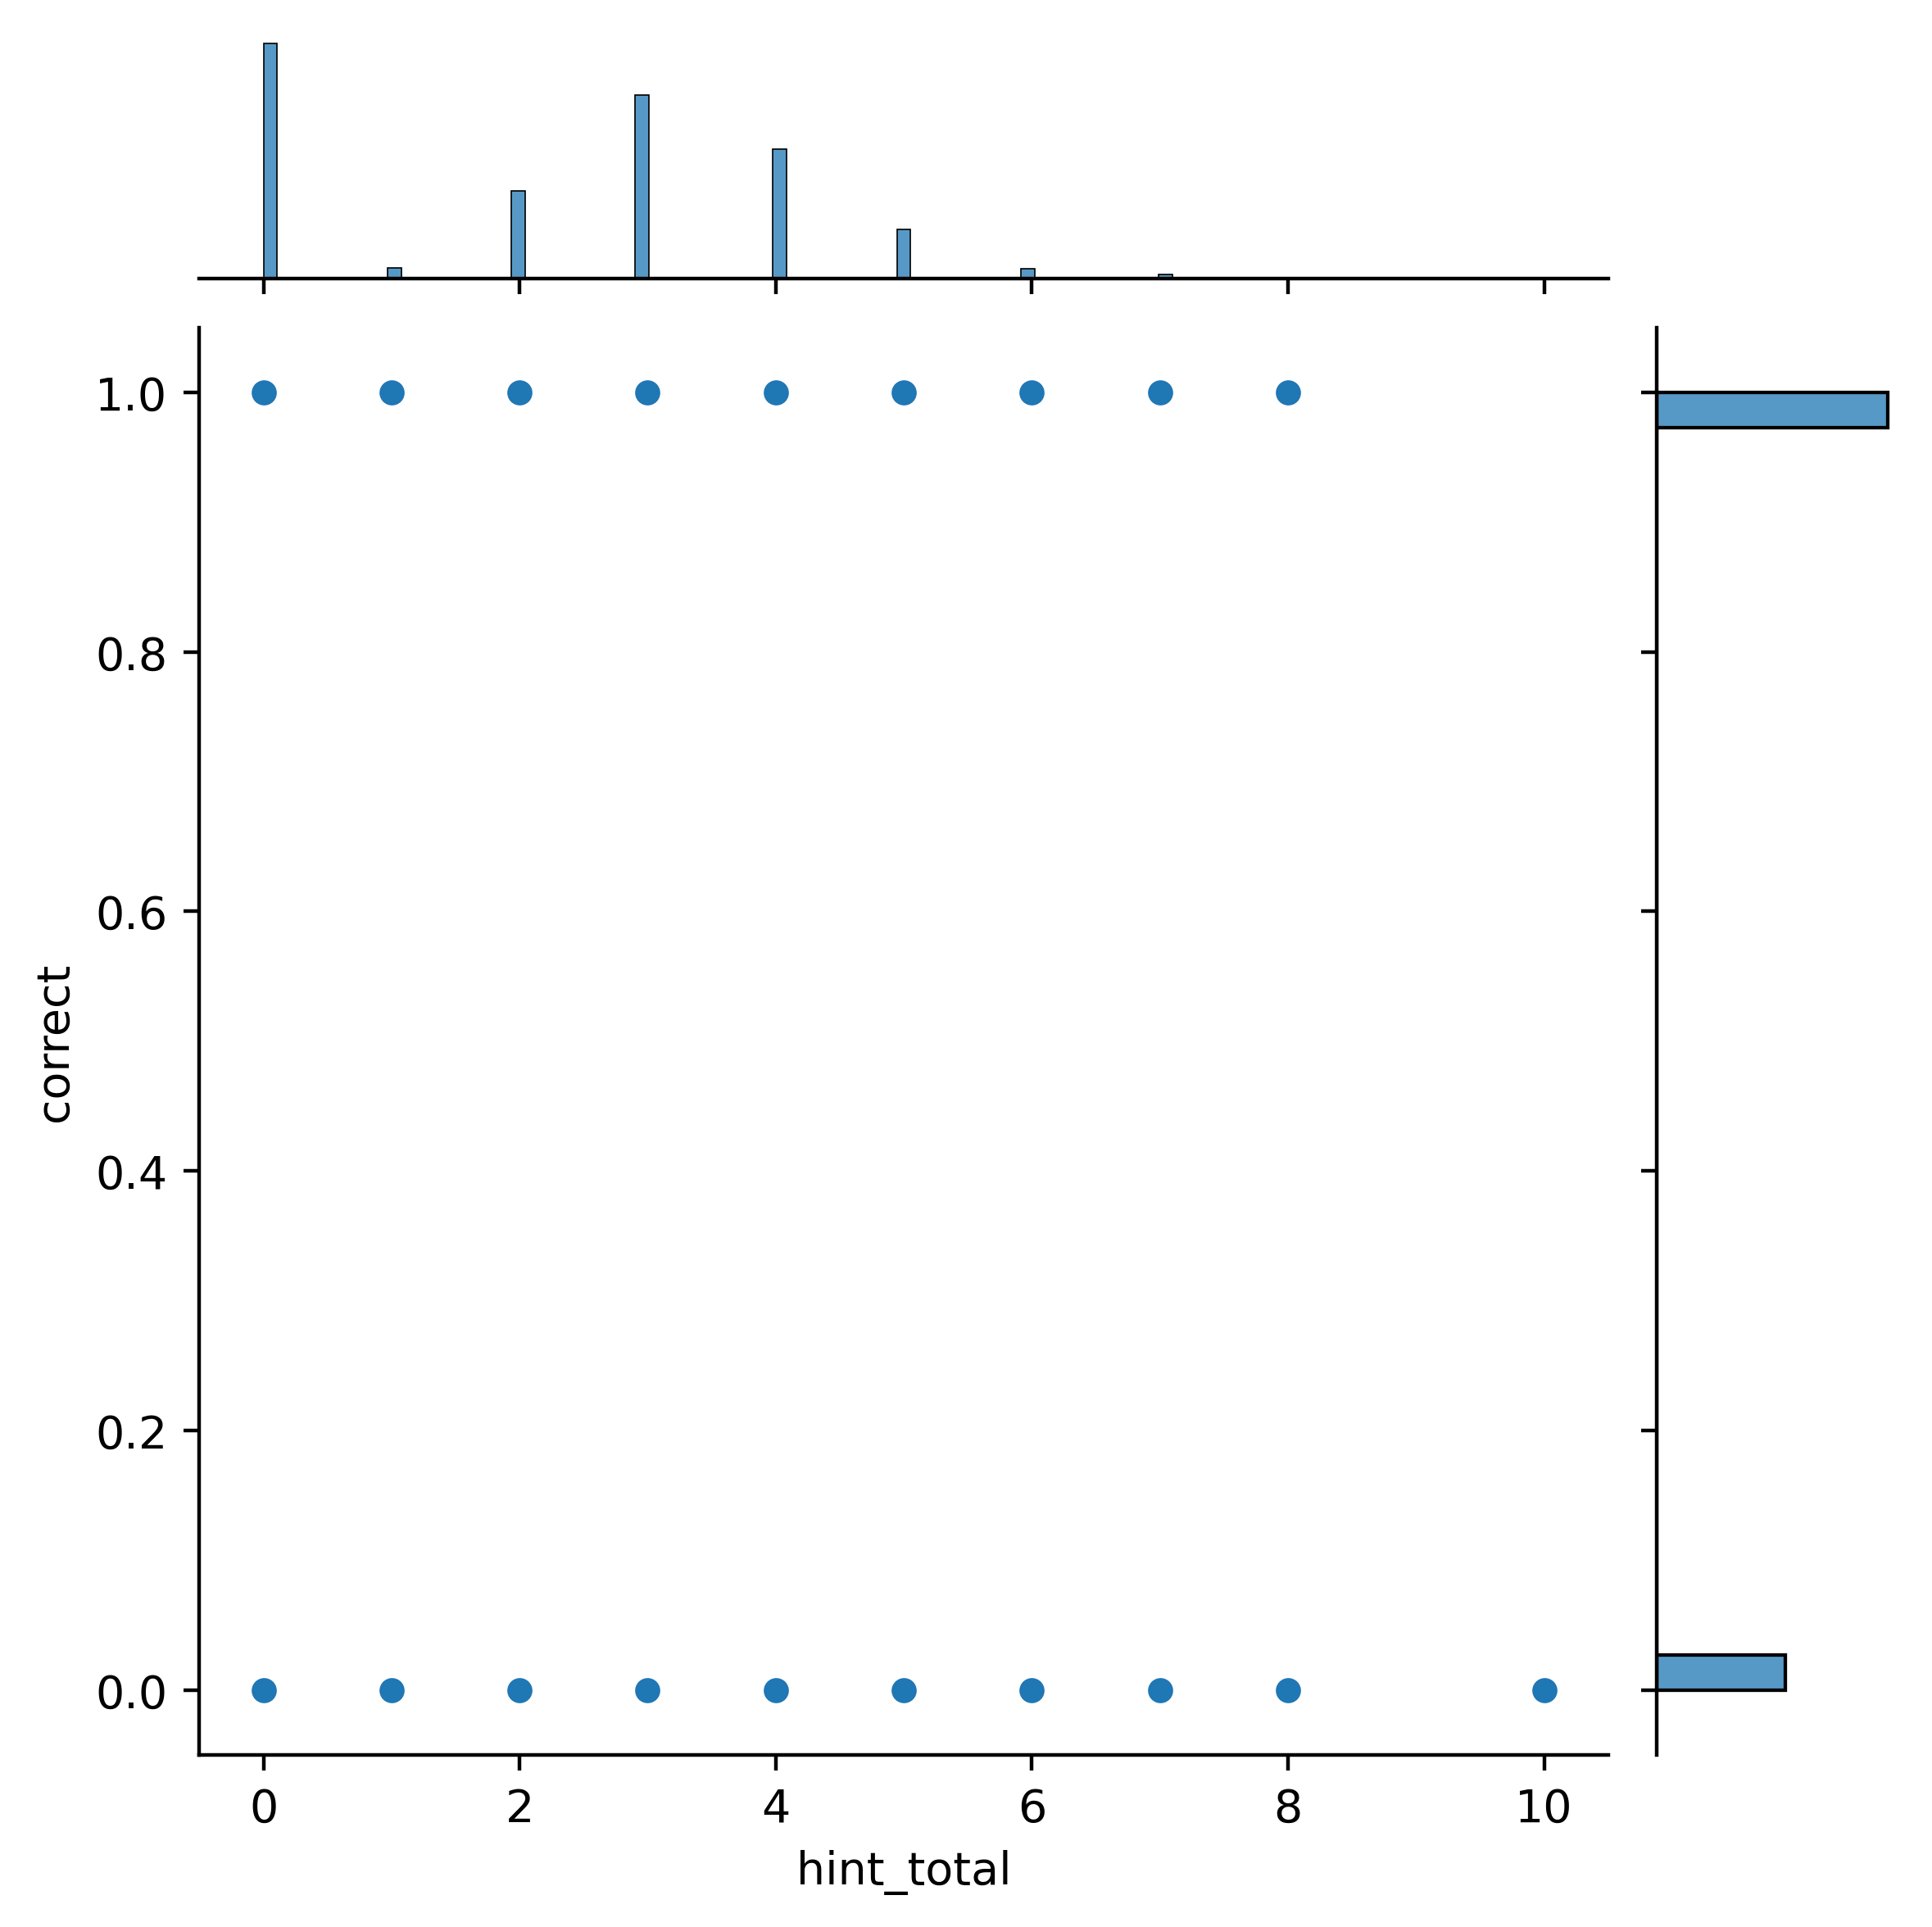
\includegraphics[width=0.9\textwidth]{ch3-jointplot-htc.png}
        \caption[dis]{The joint-plot of hint\_total}\label{fig:ch3-jointplot-htc}
    \end{subfigure}
    \begin{subfigure}[b]{0.475\textwidth}
        \centering
        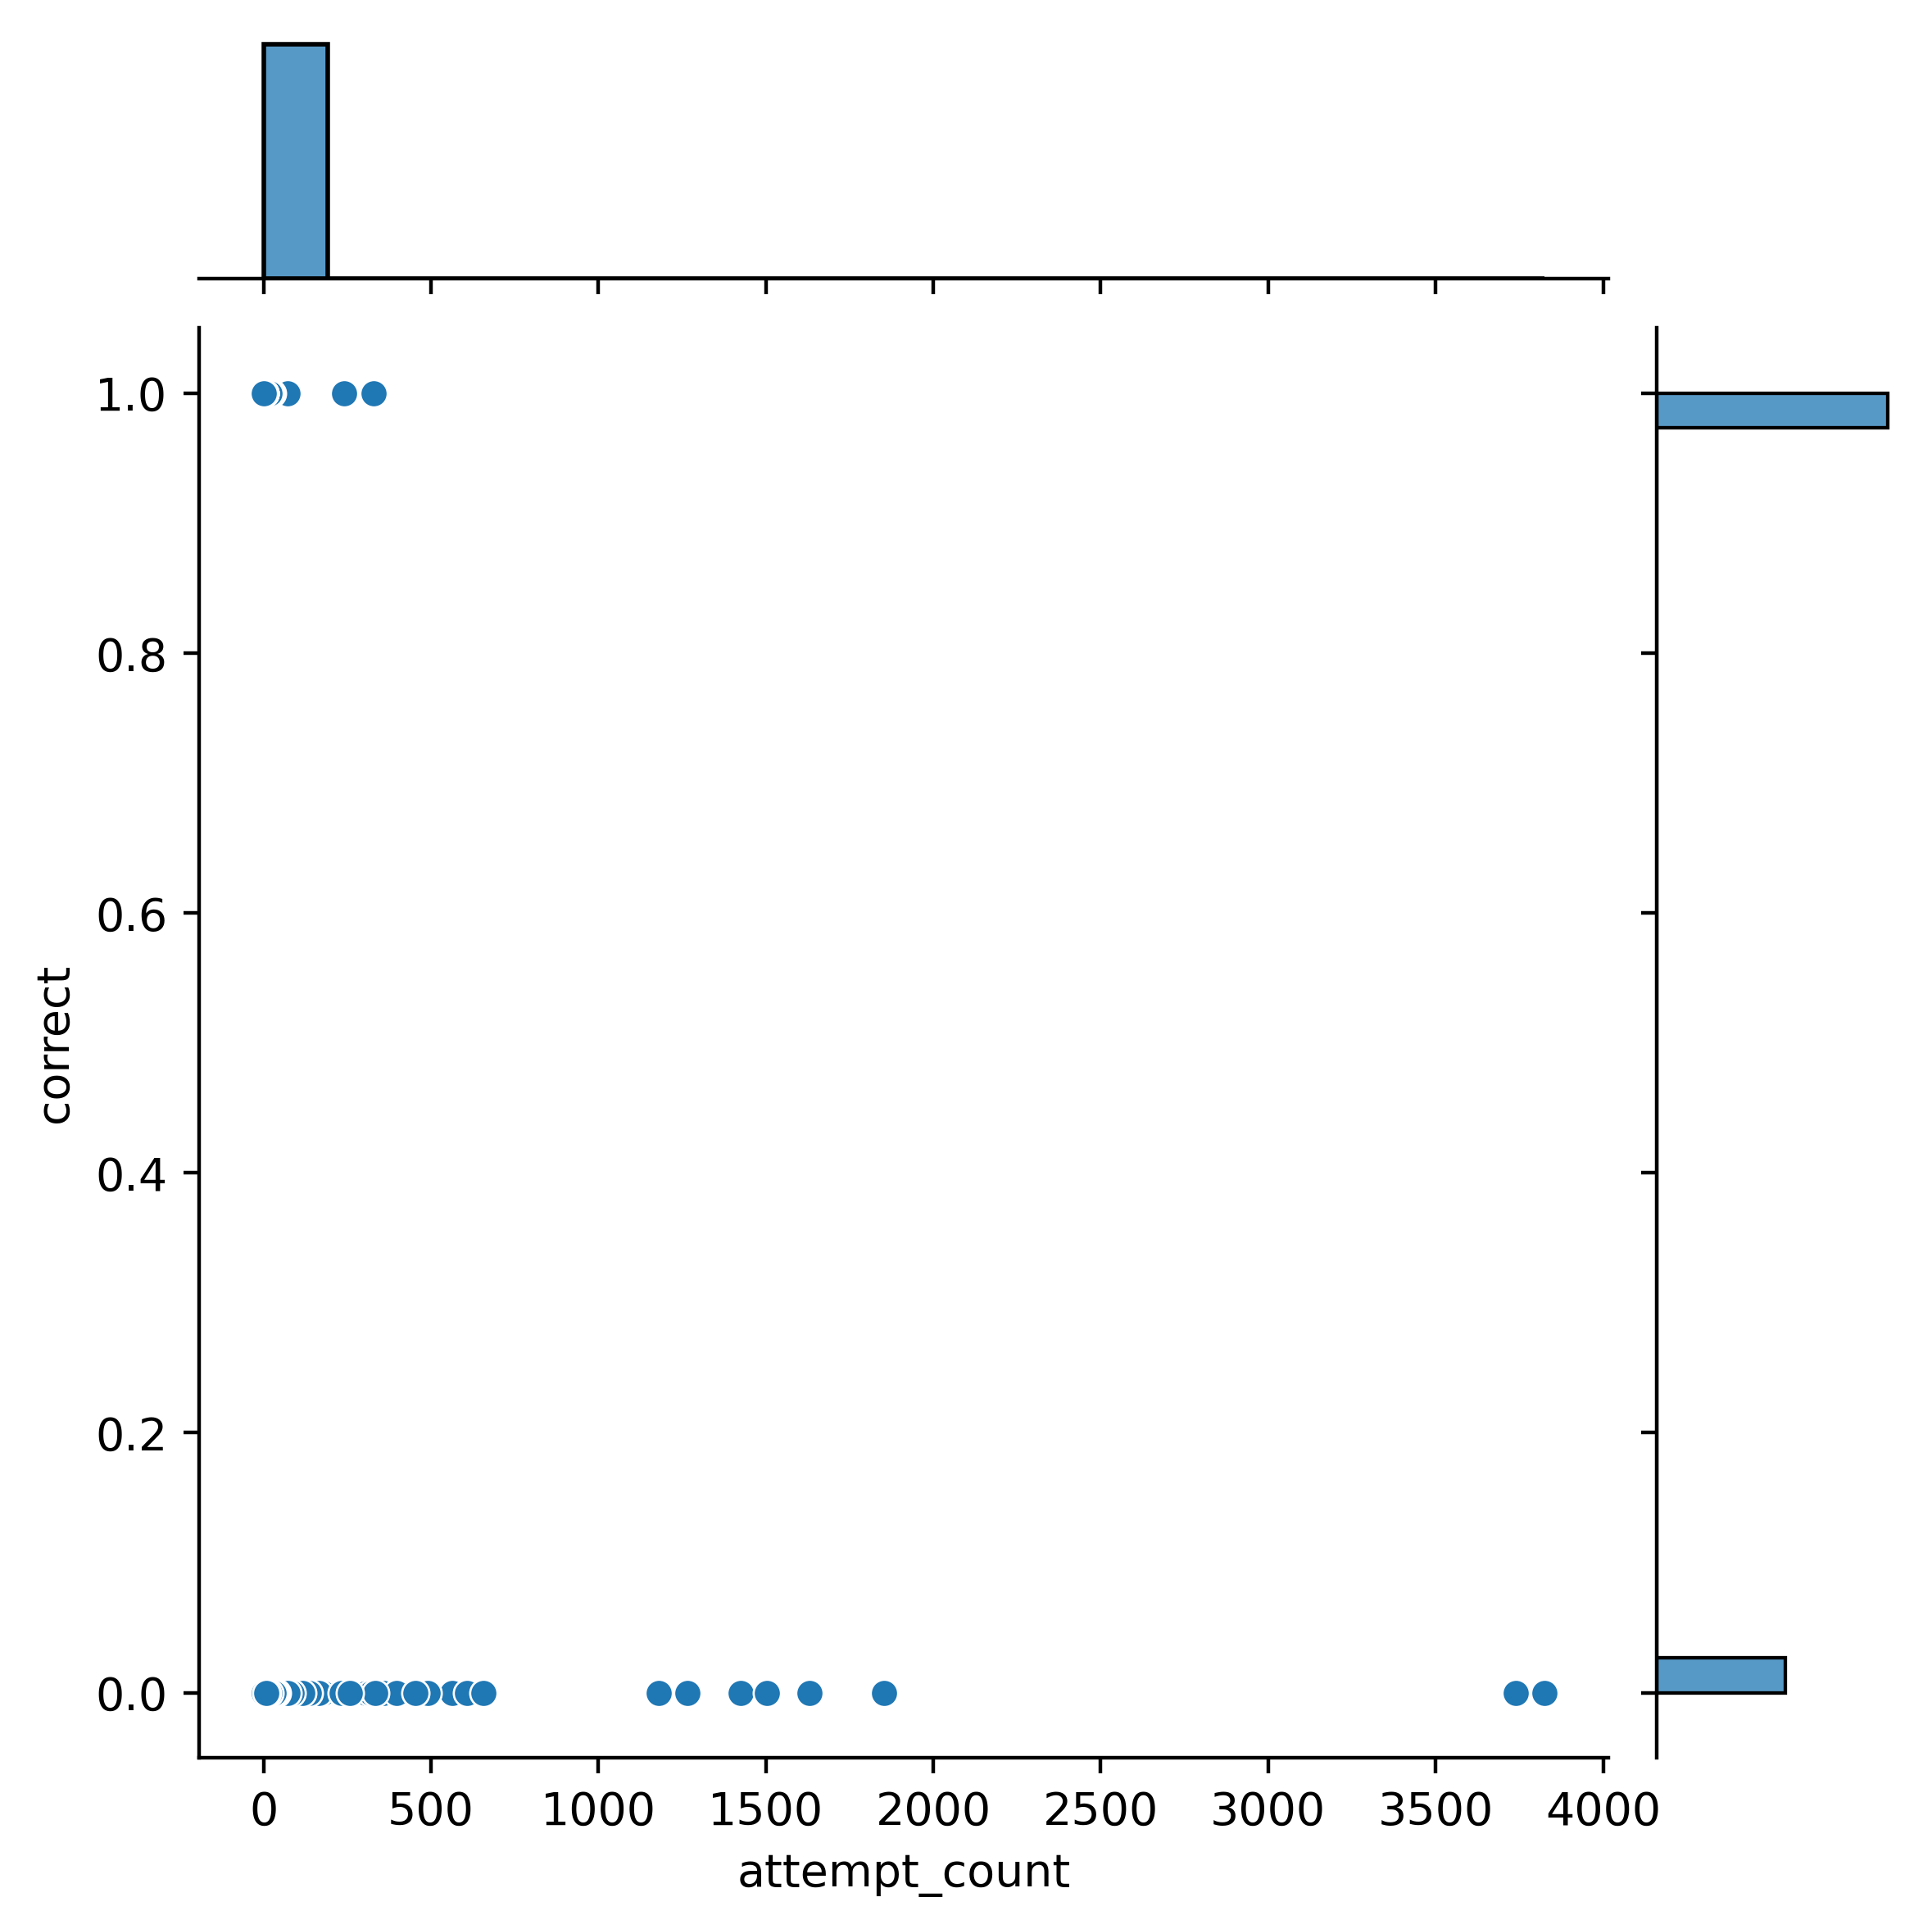
\includegraphics[width=0.9\textwidth]{ch3-jointplot-atc.png}
        \caption{The joint-plot of attempt\_count}\label{fig:ch3-jointplot-atc}
    \end{subfigure}
    \caption{The joint-plots between input features and target feature}\label{fig:ch3-jointplots}
\end{figure}

%经过上述分析,可以将上述四个特征作为模型的额外输入特征,可以作为判断最终输出的重要依据。
After the above analysis, the above four features can be used as additional input features for the model, which can be used as an important basis for judging the final output.
\subsection{Metrics}
%知识追踪本质上是一个分类问题,在机器学习领域中,常用的分类指标有Accuracy,Precision,Recall,F1 Score,AUC等。在二分类问题中,有如图\figname{\ref{fig:ch3-conmat}}的混淆矩阵,则这些分类指标的公式可以写作
Knowledge tracing is essentially a classification problem, where the commonly used classification metrics are Accuracy, Precision, Recall, F1 Score, etc. In the binary classification problem, there is the confusion matrix as shown in \figname{\ref{fig:ch3-conmat}}.
\begin{figure}[htbp!]
    \centering
    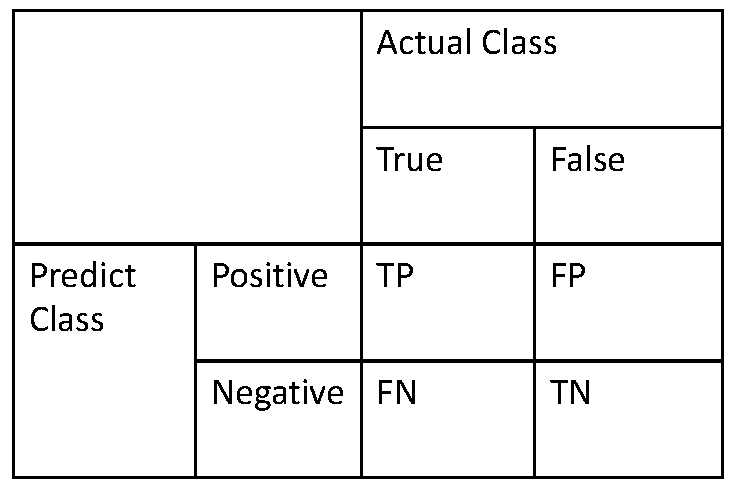
\includegraphics[width=0.85\textwidth]{ch3-conmat.pdf}
    \caption{The confusion matrix}\label{fig:ch3-conmat}
\end{figure}

Then, the formula for these classification indicators can be represented as \eqname{\ref{fml:ch3-conmat}}. The TP, TN, FP, FN represent true positive, true negative, false positive, and false negative. Although the Accuracy can determine the correct overall rate, the imbalance between positive and negative sample sizes can lead to high accuracy rates that do not fully measure the system's recognition performance for both categories. Additionally, Precision represents the proportion of true positive samples predicted as positive samples, which measures the accuracy of prediction of positive sample results, and Recall represents the bi l of true positive samples identified correctly. When Precision and Recall are plotted against each other, a P-R curve can be obtained. As Recall increases, Precision decreases overall, so a trade-off between the two is required. The F1 is a comprehensive indicator for weighing Precision and Recall.
\begin{align}\label{fml:ch3-conmat}
    \begin{split}
        \operatorname{Accuracy} &= \frac{TP+TN}{TP+TN+FP+FN} \\
        \operatorname{Precision} &= \frac{TP}{TP+FP} \\
        \operatorname{Recall} &= \frac{TP}{TP+FN} \\
        \operatorname{F1} &= \frac{2\times \operatorname{Precision}\times\operatorname{Recall}}{\operatorname{Precision}+\operatorname{Recall}}
    \end{split}
\end{align}
%为了解决样本不平衡的问题,即答对习题和答错习题量差别较大的情况,需要分别对正样本和负样本采用特定的统计特征。因此可以采取这种做法。其中\(\operatorname{TPR}=\operatorname{TP}/(\operatorname{TP}+\operatorname{FN})\)与\(\operatorname{FPR}=\operatorname{FP}/\operatorname{FP}+\operatorname{TN}\)基于实际的正样本和负样本进行统计,排除了样本不平衡的影响。FPR 表示模型虚报的响应程度,TRP表示出模型预测相应的覆盖程度。将FPR作为x轴,TPR作为y轴,则可以绘制出Receiver Operating Characteristic曲线,该曲线可以评价模型的预测能力。随着不断遍历所有的分类阈值,FPR和TPR会随着ROC曲线变动。根据上述统计量可以推知,当TPR 越高,同时 FPR 越低,ROC曲线越陡峭,那么模型的性能就越好。 它可以解决样本不平衡的问题。
To address the problem of sample imbalance, i.e., a large difference in the amount of correct and incorrect answers to an exercise, specific statistical characteristics need to be applied to the positive and negative samples, respectively. The \(\operatorname{TPR}=\operatorname{TP}/(\operatorname{TP}+\operatorname{FN})\) and \(\operatorname{FPR}=\operatorname{FP}/\operatorname{FP}+\operatorname{TN}\) based on the actual positive and negative samples can be applied for the statistics, excluding the effect of sample imbalance. \(\operatorname{FPR}\) indicates the degree of response that the model falsely reports, and \(\operatorname{TPR}\) indicates the corresponding degree of coverage predicted by the model. Taking FPR as the x-axis and TPR as the y-axis, a Receiver Operating Characteristic (ROC) curve can be plotted, which evaluates the model's predictive ability. As all the classification thresholds are traversed, the FPR and TPR will change with the ROC curve. The ROC curve is also plotted by traversing all the classification thresholds, which can solve the problem of sample imbalance. Based on the above analysis, it can be inferred that when the TPR is higher and at the same time the FPR is lower, the steeper the ROC curve is, then the performance of the model is better. It can solve the problem of sample imbalance.


%目前知识追踪领域的论文多以(Area Under Curve)AUC作为对比指标,AUC是一个基于ROC曲线常用的二分类评测手段,具有较好的性能对比能力。在知识追踪任务中,最终预测也是当前时刻的习题的做对与否,本质上为一个二分类问题,
To measure the ROC curve's steepness, Area Under Curve (AUC) can be a suitable statistic. AUC is a commonly used two-category evaluation method based on the ROC curve and has good performance comparison capabilities. The closer the AUC is to 1, the stronger the predictive performance of the model. At present, most papers in the field of knowledge tracing use AUC as a comparison indicator. In the task of knowledge tracing, the final prediction is whether the exercises at the current moment are done correctly or not, which is essentially a binary classification problem so that this approach can be adopted.

\subsection{Experiment Settings}
%本实验采用KFold方法分割测试集和验证集,取\(K=5\)。原始数据经过处理,会将每个学生的做题序列进行隔离,超过预定最长序列长度的学生会被分割成若干个不超过最长长度的序列。而实验可以采用不同的知识追踪对象进行交叉验证实验,可以有效衡量模型的预测性能。
This experiment uses the KFold method to partition the test and validation sets, taking \(K=5\). The raw data are processed to segregate the sequence of questions done by each student, and students who exceed the predetermined longest sequence length are split into several sequences that do not exceed the longest length. Moreover, the experiments can use different knowledge tracking objects for cross-validation experiments, which can effectively measure the model's prediction performance.
%本实验主要运行在深度学习服务器上,运行环境见表.

This experiment runs on a dedicated GPU computing server, and the running environment is shown in \tblname{\ref{tbl:ch3-exp-env}}.
\begin{table}[htbp!]
    \caption{Experiment running environment}\label{tbl:ch3-exp-env}
    \centering
    \begin{tabular}{l c}
        \toprule
        Software/Hardware & Configuration   \\
        \midrule
        CPU               & Xeon Gold 6139  \\
        GPU               & Tesla V100      \\
        VRAM              & 16G             \\
        Operating System  & Ubuntu 18.04    \\
        Python            & 3.8.6           \\
        PyTorch           & 1.8.0           \\
        GPU Driver        & Cuda11.2/cudnn8 \\
        \bottomrule
    \end{tabular}
\end{table}


\subsection{Baselines}
%1.BKT是一个知识追踪的经典模型,它基于隐马尔可夫模型(HMM),将学习者的知识状态建模为一组对应知识点掌握情况的二元变量。
%2.DKT是第一个基于深度学习的知识追踪模型,它应用将学生的做题记录输入到LSTM中,可以捕获学生做题序列上近期做题记录的影响,将学生的做题顺序考虑进模型,DKT也初步考虑了知识点间的内在相关性。
%3.GKT应用图神经网络到知识追踪任务上,利用图的特性,将知识点间的图状关联表征出来,从而更好地学习知识内在依赖关系,该模型能够学习出学生的隐藏知识状态,也具有较好的可解释性。
In this experiment, baseline performance comparisons are made by comparing some classic models with new knowledge tracing models proposed recently. The following models participate in performance comparison.
\begin{itemize}
    \item Deep knowledge tracing~\cite{piech2015deep}: DKT applies the input of students' doing records into LSTM and can capture the influence of recent doing records on students' doing sequences, taking students' doing sequences into account into the model; DKT also initially considers the intrinsic correlation between knowledge points.
    \item Dynamic key-value memory networks (DKVMN)~\cite{zhang2017dynamic}: DKVMN uses key-value pairs as the memory structure, which can avoid over better prediction performance relative to BKT, and DKT is achieved by using key-value pairs as the memory structure.
    \item Self-attentive model for knowledge tracing (SAKT)~\cite{sakt2019}: The SAKT model takes into account the correlation between exercises in terms of potential knowledge points, and introduces the Transformer structure to calculate the attention between input sequences of exercises, so that the relevance of current exercises can be calculated based on previous exercises and reasonable predictions can be made.
    \item Neural pedagogical agent (NPA)~\cite{Lee2019CreatingAN}: NPA applied Attention based Bi-LSTM model to knowledge tracing task, which takes into account the bidirectional information of the question-answering sequence, and the subsequent answer sequence interactions also correct the previous predictions.
\end{itemize}

\subsection{Model Training}
%本模型需要预定义一些训练参数,经过参数调整,得到如表\figname{\ref{tbl:ch3-hpsetting}}所示的参数组合
This model requires some predefined training parameters, and after parameter adjustment, the parameter combinations shown in \tblname{\ref{tbl:ch3-hpsetting}} are obtained.
\begin{table}[htbp!]
    \caption{Hyperparameter settings of proposed model}\label{tbl:ch3-hpsetting}
    \centering
    \begin{tabular}{l c c}
        \toprule
        Hyperparameter & Description                             & Value \\
        \midrule
        lr             & learning rate                           & 0.01  \\
        opt            & optimizer                               & Adam  \\
        batch\_size    & batch size                              & 32    \\
        maxseqlen      & maximum sequence length                 & 200   \\
        q\_embed\_dim  & exercise embedding dimension            & 50    \\
        qa\_embed\_dim & exercise  answering embedding dimension & 20    \\
        memory\_size   & number of memory slots                  & 20    \\
        \bottomrule
    \end{tabular}
\end{table}
%实验总共进行了三次训练,选取了平均的训练过程参数进行训练数据图绘制,得到损失训练图和模型性能训练图,如图所示。
The experiments were conducted a total of three times, and the average training output was selected for training data plotting to obtain the loss training plot and the model performance training plot, as shown in \figname{\ref{fig:ch3-train-loss}} and \figname{\ref{fig:ch3-train-acc}}.
\begin{figure}[htbp!]
    \centering
    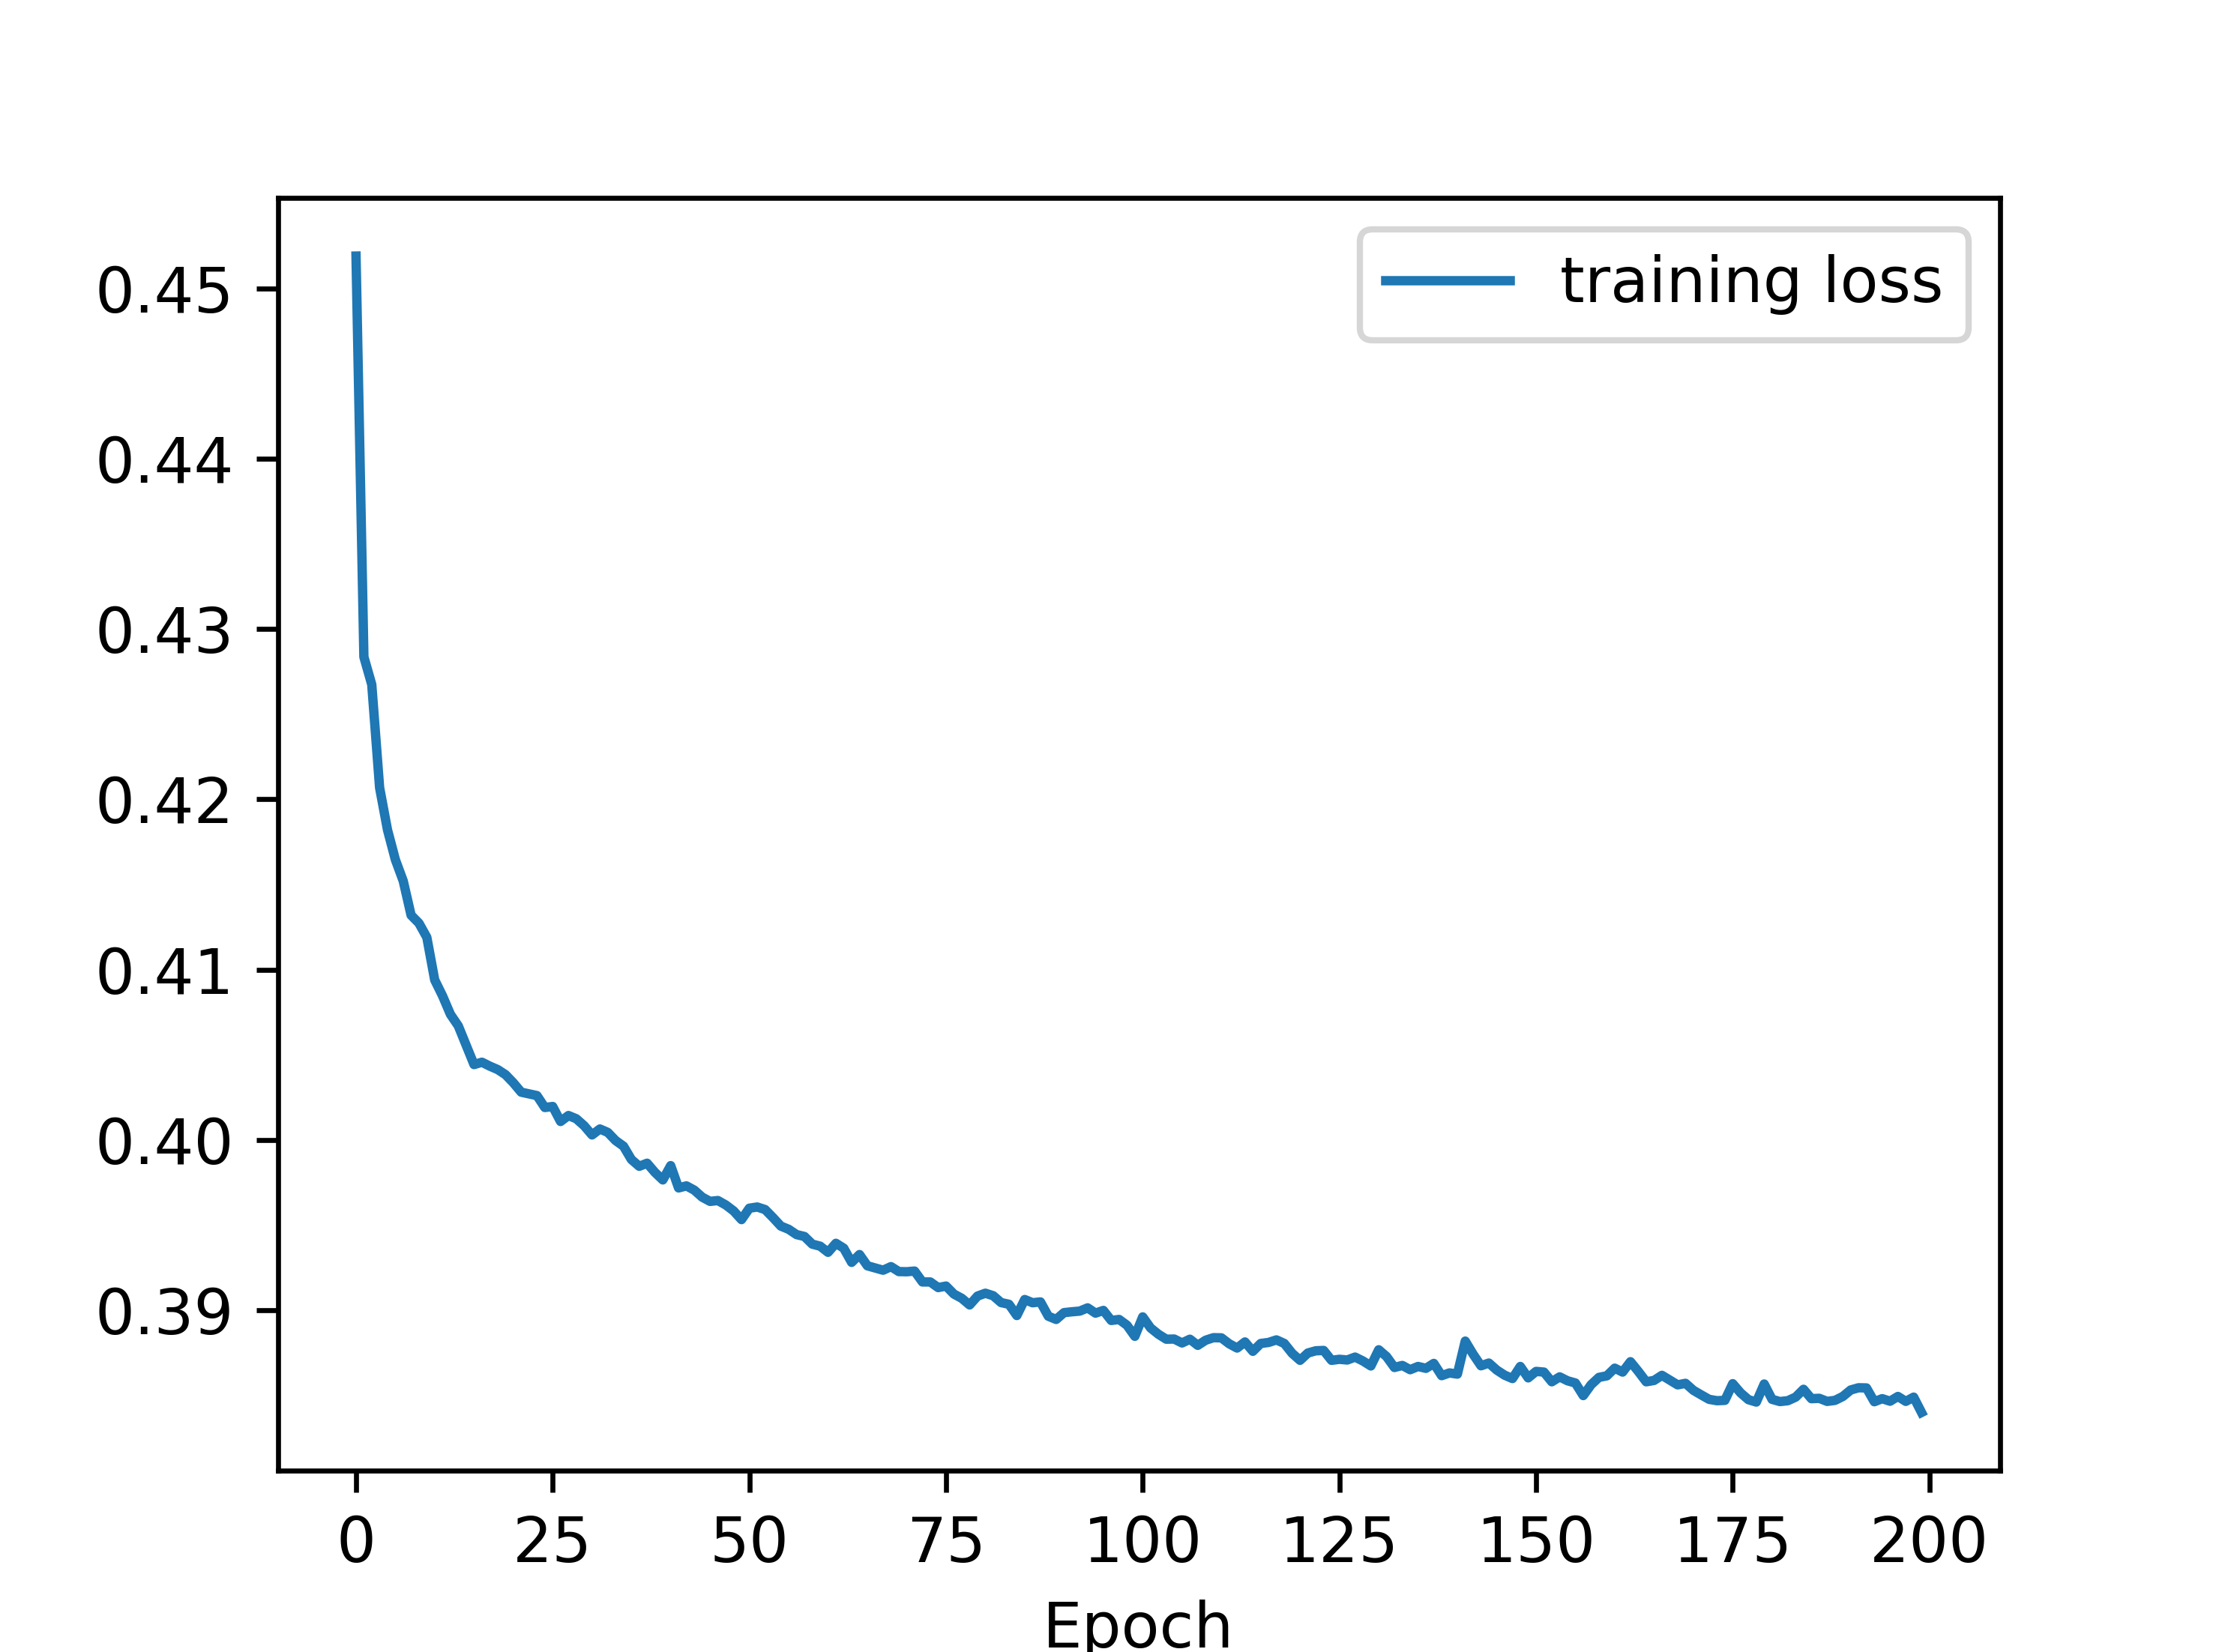
\includegraphics[width=0.9\textwidth]{ch3-train-loss.png}
    \caption{The training process of proposed model}\label{fig:ch3-train-loss}
\end{figure}

\begin{figure}[htb]
    \centering
    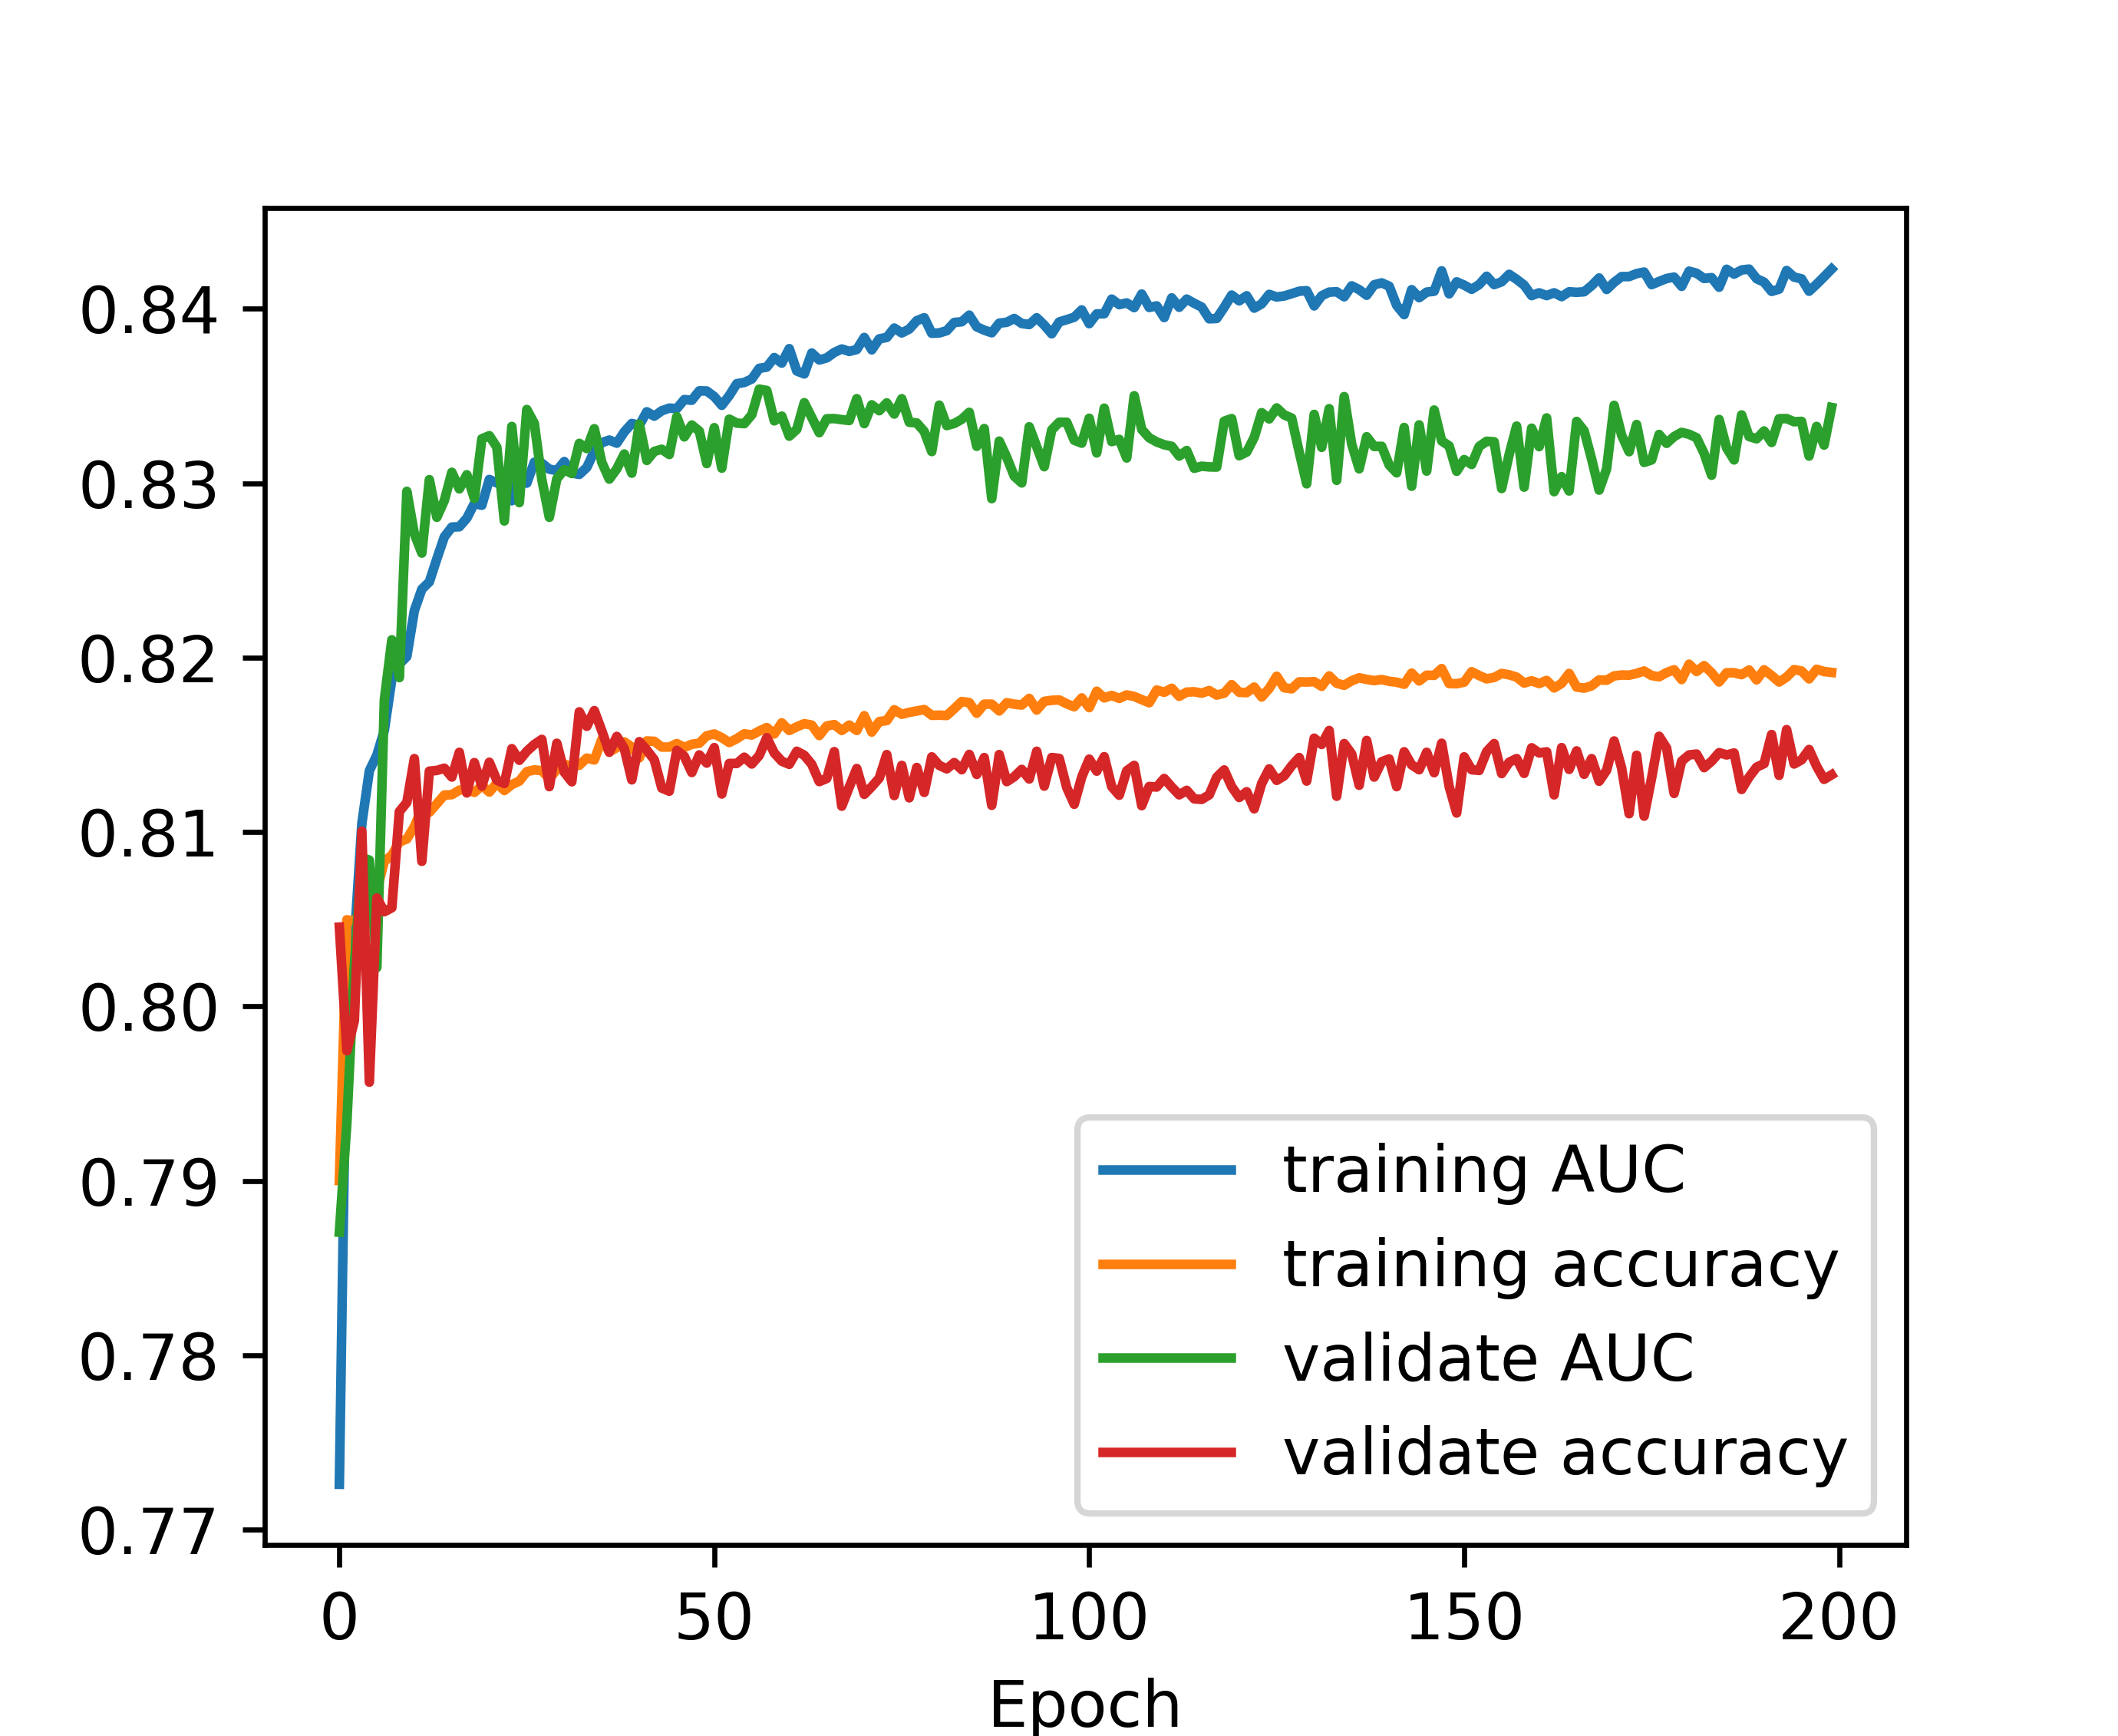
\includegraphics[width=0.9\textwidth]{ch3-train-acc.png}
    \caption{The training acc/auc of proposed model}\label{fig:ch3-train-acc}
\end{figure}
%结果显示,经过约150个epoch的训练,模型的预测性能可以稳定收敛。

The results show that the model's prediction performance can converge stably after about 150 epochs of training.
\subsection{Result and Analysis}
%实验结果见表\cite{\ref{tbl:ch3-performance}},相比于其他模型,提出的模型的性能在关键指标accuracy和AUC取得了最优的指标。有两点原因,一是因为模型考虑了用户的额外特征,因此引入了新的影响因素,二是模型考虑了潜在概念之间的模型,并利用图状结构来表征这种联系,从而为模型引入了高阶的知识点关系特征。综上所述,模型为知识追踪任务引入了新的解释特征,因此在模型的最终性能指标上取得了较大的提升。
The experimental results are presented in \tblname{\ref{tbl:ch3-performance}}, and the performance of the proposed model achieves optimal metrics in key indicators accuracy and AUC compared to other models. There are two reasons for this, one is because the model considers additional features of the user and therefore introduces new influencing factors, and the other is that the model considers the model between potential concepts and uses graph-like structures to characterize such connections, thus introducing higher-order knowledge point relationship features to the model. In summary, the model introduces new explanatory features for the knowledge tracking task and therefore achieves a large improvement in the final performance metrics of the model.

\begin{table}[htb]
    \centering
    \caption{Performance comparison between baseline and proposed models}\label{tbl:ch3-performance}
    \begin{tabular}{cccc}
        \toprule
        Model    & ACC (\%)                    & AUC (\%)                   & Training time (sec) \\
        \midrule
        DKT      & \(76.99\pm 0.08 \)          & \(81.79\pm 0.09\)          & \(2,731\)           \\
        DKVMN    & \(75.63\pm 0.19 \)          & \(79.58\pm 0.27\)          & \(3,378\)           \\
        NPA      & \(77.09\pm 0.08\)           & \(81.81\pm 0.13\)          & \(3,872\)           \\
        SAKT     & \(76.37\pm 0.15\)           & \(80.77\pm 0.09\)          & \(4,367\)           \\
        \midrule
        Proposed & \(\mathbf{81.34\pm 0.25} \) & \(\mathbf{83.20\pm 0.25}\) & \(4,597\)           \\
        \bottomrule
    \end{tabular}
\end{table}

%而在模型训练耗时上,本模型由于需要额外的图信息传播过程,因此相较于原始DKVMN模型训练效率会有所降低,为了解决该问题,可以考虑将图传播的方式通过矩阵运算的方式来进行计算,可以充分利用计算设备并行计算的能力。
As for the model training time consumption, this model will have a reduced training efficiency compared to the original DKVMN model because of the additional graph information propagation process. To solve this problem, the graph propagation can be considered to be computed by means of matrix operations, which can make full use of the parallel computing capability of computing devices.
\section{Summary}
In this section, an improved GKVMN model based on DKVMN is proposed, which adds the ability to characterize the relationships between knowledge points to the model by transforming the storage module that characterizes the potential concepts of the exercises into a graph structure. On the other hand, the model introduces the student's answer characteristics to introduce more influencing factors, thus enhancing the predictive power for the model. In addition, the value storage module of the model can be used as the student's knowledge point mastery representation, which can explicitly output the student's mastery of potential concepts, thus adding more recommended input features for the subsequent exercise recommendation.

The main contributions of this section are as follows.
\begin{enumerate}
    \item the graph structure is used to characterize the relationship between the potential concepts of the exercises, taking into account the impact of the increase in mastery of the relevant knowledge points on the overall knowledge mastery. A graph propagation calculation is used to characterize the change in mastery of the relevant knowledge points.
    \item additional student characteristics are introduced as inputs to the model, which adds more predictors to the model and takes into account the impact of various situations on the final correctness of the answers.
    \item the knowledge mastery proficiency of the model can be output explicitly, which improves the interpretability of the model.
\end{enumerate}

%在实验阶段,首先对原始数据集进行数据清洗、格式转换,然后对数据集进行特征相关性分析,目标-特征相关性分析,选取最佳的学生答题特征作为额外的输入特征。然后与一系列baseline知识追踪模型进行性能对比。实验显示,提出的模型在各项指标上都优于基线模型。
In the experimental phase, the original dataset is firstly cleaned and formatted with data, and then the dataset is analyzed with feature correlation analysis and target-feature correlation analysis to select the best student answer features as additional input features. Then the performance is compared with a series of baseline knowledge tracking models. The experiments show that the proposed model outperforms the baseline model in all metrics.